% Options for packages loaded elsewhere
\PassOptionsToPackage{unicode}{hyperref}
\PassOptionsToPackage{hyphens}{url}
\PassOptionsToPackage{dvipsnames,svgnames,x11names}{xcolor}
%
\documentclass[
]{article}

\usepackage{amsmath,amssymb}
\usepackage{iftex}
\ifPDFTeX
  \usepackage[T1]{fontenc}
  \usepackage[utf8]{inputenc}
  \usepackage{textcomp} % provide euro and other symbols
\else % if luatex or xetex
  \usepackage{unicode-math}
  \defaultfontfeatures{Scale=MatchLowercase}
  \defaultfontfeatures[\rmfamily]{Ligatures=TeX,Scale=1}
\fi
\usepackage{lmodern}
\ifPDFTeX\else  
    % xetex/luatex font selection
\fi
% Use upquote if available, for straight quotes in verbatim environments
\IfFileExists{upquote.sty}{\usepackage{upquote}}{}
\IfFileExists{microtype.sty}{% use microtype if available
  \usepackage[]{microtype}
  \UseMicrotypeSet[protrusion]{basicmath} % disable protrusion for tt fonts
}{}
\makeatletter
\@ifundefined{KOMAClassName}{% if non-KOMA class
  \IfFileExists{parskip.sty}{%
    \usepackage{parskip}
  }{% else
    \setlength{\parindent}{0pt}
    \setlength{\parskip}{6pt plus 2pt minus 1pt}}
}{% if KOMA class
  \KOMAoptions{parskip=half}}
\makeatother
\usepackage{xcolor}
\usepackage[top = 1in,bottom = 1in,left = 1in,right = 1in]{geometry}
\setlength{\emergencystretch}{3em} % prevent overfull lines
\setcounter{secnumdepth}{-\maxdimen} % remove section numbering
% Make \paragraph and \subparagraph free-standing
\makeatletter
\ifx\paragraph\undefined\else
  \let\oldparagraph\paragraph
  \renewcommand{\paragraph}{
    \@ifstar
      \xxxParagraphStar
      \xxxParagraphNoStar
  }
  \newcommand{\xxxParagraphStar}[1]{\oldparagraph*{#1}\mbox{}}
  \newcommand{\xxxParagraphNoStar}[1]{\oldparagraph{#1}\mbox{}}
\fi
\ifx\subparagraph\undefined\else
  \let\oldsubparagraph\subparagraph
  \renewcommand{\subparagraph}{
    \@ifstar
      \xxxSubParagraphStar
      \xxxSubParagraphNoStar
  }
  \newcommand{\xxxSubParagraphStar}[1]{\oldsubparagraph*{#1}\mbox{}}
  \newcommand{\xxxSubParagraphNoStar}[1]{\oldsubparagraph{#1}\mbox{}}
\fi
\makeatother


\providecommand{\tightlist}{%
  \setlength{\itemsep}{0pt}\setlength{\parskip}{0pt}}\usepackage{longtable,booktabs,array}
\usepackage{calc} % for calculating minipage widths
% Correct order of tables after \paragraph or \subparagraph
\usepackage{etoolbox}
\makeatletter
\patchcmd\longtable{\par}{\if@noskipsec\mbox{}\fi\par}{}{}
\makeatother
% Allow footnotes in longtable head/foot
\IfFileExists{footnotehyper.sty}{\usepackage{footnotehyper}}{\usepackage{footnote}}
\makesavenoteenv{longtable}
\usepackage{graphicx}
\makeatletter
\newsavebox\pandoc@box
\newcommand*\pandocbounded[1]{% scales image to fit in text height/width
  \sbox\pandoc@box{#1}%
  \Gscale@div\@tempa{\textheight}{\dimexpr\ht\pandoc@box+\dp\pandoc@box\relax}%
  \Gscale@div\@tempb{\linewidth}{\wd\pandoc@box}%
  \ifdim\@tempb\p@<\@tempa\p@\let\@tempa\@tempb\fi% select the smaller of both
  \ifdim\@tempa\p@<\p@\scalebox{\@tempa}{\usebox\pandoc@box}%
  \else\usebox{\pandoc@box}%
  \fi%
}
% Set default figure placement to htbp
\def\fps@figure{htbp}
\makeatother
% definitions for citeproc citations
\NewDocumentCommand\citeproctext{}{}
\NewDocumentCommand\citeproc{mm}{%
  \begingroup\def\citeproctext{#2}\cite{#1}\endgroup}
\makeatletter
 % allow citations to break across lines
 \let\@cite@ofmt\@firstofone
 % avoid brackets around text for \cite:
 \def\@biblabel#1{}
 \def\@cite#1#2{{#1\if@tempswa , #2\fi}}
\makeatother
\newlength{\cslhangindent}
\setlength{\cslhangindent}{1.5em}
\newlength{\csllabelwidth}
\setlength{\csllabelwidth}{3em}
\newenvironment{CSLReferences}[2] % #1 hanging-indent, #2 entry-spacing
 {\begin{list}{}{%
  \setlength{\itemindent}{0pt}
  \setlength{\leftmargin}{0pt}
  \setlength{\parsep}{0pt}
  % turn on hanging indent if param 1 is 1
  \ifodd #1
   \setlength{\leftmargin}{\cslhangindent}
   \setlength{\itemindent}{-1\cslhangindent}
  \fi
  % set entry spacing
  \setlength{\itemsep}{#2\baselineskip}}}
 {\end{list}}
\usepackage{calc}
\newcommand{\CSLBlock}[1]{\hfill\break\parbox[t]{\linewidth}{\strut\ignorespaces#1\strut}}
\newcommand{\CSLLeftMargin}[1]{\parbox[t]{\csllabelwidth}{\strut#1\strut}}
\newcommand{\CSLRightInline}[1]{\parbox[t]{\linewidth - \csllabelwidth}{\strut#1\strut}}
\newcommand{\CSLIndent}[1]{\hspace{\cslhangindent}#1}

\usepackage{orcidlink}
\usepackage{marvosym}
\usepackage{xcolor}
\usepackage{marginnote}
\reversemarginpar
\newcommand{\paragraphnumber}[1]{\marginnote{\color{lightgray}\tiny{#1}}[0pt]}
\makeatletter
\@ifpackageloaded{tcolorbox}{}{\usepackage[skins,breakable]{tcolorbox}}
\@ifpackageloaded{fontawesome5}{}{\usepackage{fontawesome5}}
\definecolor{quarto-callout-color}{HTML}{909090}
\definecolor{quarto-callout-note-color}{HTML}{0758E5}
\definecolor{quarto-callout-important-color}{HTML}{CC1914}
\definecolor{quarto-callout-warning-color}{HTML}{EB9113}
\definecolor{quarto-callout-tip-color}{HTML}{00A047}
\definecolor{quarto-callout-caution-color}{HTML}{FC5300}
\definecolor{quarto-callout-color-frame}{HTML}{acacac}
\definecolor{quarto-callout-note-color-frame}{HTML}{4582ec}
\definecolor{quarto-callout-important-color-frame}{HTML}{d9534f}
\definecolor{quarto-callout-warning-color-frame}{HTML}{f0ad4e}
\definecolor{quarto-callout-tip-color-frame}{HTML}{02b875}
\definecolor{quarto-callout-caution-color-frame}{HTML}{fd7e14}
\makeatother
\makeatletter
\@ifpackageloaded{caption}{}{\usepackage{caption}}
\AtBeginDocument{%
\ifdefined\contentsname
  \renewcommand*\contentsname{Table of contents}
\else
  \newcommand\contentsname{Table of contents}
\fi
\ifdefined\listfigurename
  \renewcommand*\listfigurename{List of Figures}
\else
  \newcommand\listfigurename{List of Figures}
\fi
\ifdefined\listtablename
  \renewcommand*\listtablename{List of Tables}
\else
  \newcommand\listtablename{List of Tables}
\fi
\ifdefined\figurename
  \renewcommand*\figurename{Figure}
\else
  \newcommand\figurename{Figure}
\fi
\ifdefined\tablename
  \renewcommand*\tablename{Table}
\else
  \newcommand\tablename{Table}
\fi
}
\@ifpackageloaded{float}{}{\usepackage{float}}
\floatstyle{ruled}
\@ifundefined{c@chapter}{\newfloat{codelisting}{h}{lop}}{\newfloat{codelisting}{h}{lop}[chapter]}
\floatname{codelisting}{Listing}
\newcommand*\listoflistings{\listof{codelisting}{List of Listings}}
\makeatother
\makeatletter
\makeatother
\makeatletter
\@ifpackageloaded{caption}{}{\usepackage{caption}}
\@ifpackageloaded{subcaption}{}{\usepackage{subcaption}}
\makeatother

\usepackage{bookmark}

\IfFileExists{xurl.sty}{\usepackage{xurl}}{} % add URL line breaks if available
\urlstyle{same} % disable monospaced font for URLs
\hypersetup{
  pdftitle={Locating Creative Agency in Archaeological Data Work},
  pdfauthor={Zachary Batist},
  pdfkeywords={data work, information infrastructures, fieldwork
practices},
  colorlinks=true,
  linkcolor={blue},
  filecolor={Maroon},
  citecolor={Blue},
  urlcolor={Blue},
  pdfcreator={LaTeX via pandoc}}


\title{Locating Creative Agency in Archaeological Data Work}

\author{
      {Zachary
Batist \orcidlink{0000-0003-0435-508X} \href{mailto:zachary.batist@mcgill.ca}{\Letter}} \\
          McGill University
     \\
  }

\date{2025-08-05}
\begin{document}
\maketitle
\begin{abstract}
The workflows that are now commonplace across archaeological projects
mask social and epistemic structures and principles. More specifically,
they re-distribute creative agency to promote specific kinds of outcomes
based on discrete data models. This paper draws attention to the
mechanisms through which data are created and curated, focusing on the
social and technical apparatus through which archaeologists control the
creation and flow of information. Based on observations of and
elicitations about archaeological data work in fieldwork settings at two
cases, I articulate how the management of data and of labour are
inherently intertwined, and how workflows are operationalized by
managerial systems to ensure that data are created and curated toward
productive ends. This paper therefore contributes to ongoing
theory-building and prompts further reflection on the roles of
information objects, infrastructures and professional relationships that
mediate the valuation, validation and legitimization of archaeological
knowledge.
\end{abstract}


\begin{tcolorbox}[enhanced jigsaw, colback=white, left=2mm, colframe=quarto-callout-note-color-frame, opacityback=0, arc=.35mm, bottomrule=.15mm, toprule=.15mm, title=\textcolor{quarto-callout-note-color}{\faInfo}\hspace{0.5em}{Note}, opacitybacktitle=0.6, breakable, colbacktitle=quarto-callout-note-color!10!white, toptitle=1mm, bottomtitle=1mm, leftrule=.75mm, coltitle=black, titlerule=0mm, rightrule=.15mm]

This is a preprint of a paper submitted for open peer-review through
\href{https://archaeo.peercommunityin.org/}{Peer Community in
Archaeology}. It is identical to the version archived at
\href{https://hcommons.org/}{Knowledge Commons} (DOI:
\href{https://doi.org/10.17613/8eqy4-n1m82}{10.17613/8eqy4-n1m82}).

\end{tcolorbox}

\section{Introduction}\label{introduction}

A\paragraphnumber{[1]} general tension exists between the need to
operationalize archaeological data as stable and concrete records about
the past, and a prevalent intuitive understanding of their constructed
and situated nature (Wylie 2017: 55-57; Lucas 2019: 274-278; Huggett
2022). While data serve as the evidential basis upon which analysis and
interpretation are based, they are also the products of targeted
scientific intervention and are limited by practical and methodological
constraints (Dallas 2015). Archaeologists have developed workflows as
ways of limiting archaeologists' behaviours while collecting and working
with data in order to emphasize the data's concreteness. While these
workflows are meant to systematize data work by de-personalizing the
archaeological encounter, close analysis of these protocols actually
reinforces the notion that data are the products of human decisions and
actions, and that data are constructed in relation to human needs,
desires and values (Knorr Cetina 1999, 2001).

This\paragraphnumber{[2]} paper responds to recent calls by
archaeologists who develop systematic and critical analysis of
archaeological practice and infrastructures to interrogate the apparatus
of archaeological knowledge production by examining the social and
technical mechanisms through which archaeologists control the creation
and flow of information (Huggett 2022; Dallas 2015). Through empirical
observation and analysis of archaeological work practices and of the
media and organizational structures that scaffold them, I articulate how
the managerial imperative to model behaviour according to formal
processes effectively relocates creative agency --- which constitutes
the ability and authority to set the standard against which meanings are
attributed to archaeological objects --- away from those who do the work
and toward those who direct labour and design information management
protocols. I draw from my own experiences as an archaeologist and as a
scholar of scientific practice and infrastructure to frame some common
experiences and anxieties in ways that reveal key systemic issues, which
many archaeologists struggle to articulate independently in a systematic
and rigorous manner. This work therefore contributes to ongoing
theory-building and prompts further reflection on the roles of
information objects, infrastructures and professional relationships that
mediate the valuation, validation and legitimization of archaeological
knowledge.

\section{Background}\label{background}

I\paragraphnumber{[3]} consider data as mediating devices that support
research by connecting experiences distributed across time, place and
community. Data work therefore comprises acts of collaboration, or means
of communicating varied archaeological encounters among invested
stakeholders. In other words, I conceive data work, which is omnipresent
in all aspects of archaeological research, as the transformation of
meanings from one set of activities to another via the materialization
of information objects, such as recording sheets, reports, diagrams,
finds bags, tags, scrap notes, descriptive monologues, stories,
demonstrations, among many other entities exhibiting various degrees of
tangibility and stability.

As\paragraphnumber{[4]} with all acts of communication, archaeologists
who work with data must reconcile the circumstances under which the data
were created with the potential outcomes that they desire and deem
feasible to achieve through them. As such, working with data involves
participating as part of a continuum of practice, whereby one's work is
impacted by prior actions and has the potential to influence future
outcomes (Dallas 2015: 190). I frame these connections as collaborative
commitments, which govern professional relations among members of
research communities, namely with regards to who may create and access
data and in what ways. In other words, collaborative commitments embody
the systemic norms regarding the meaningfulness of various kinds of work
and of the functional value of their information outcomes. This suits my
interest in articulating the ways in which expressions of archaeological
meaning are valued, how information systems are established to ensure
that archaeologists create information objects that exhibit such value.

This\paragraphnumber{[5]} has implications for how we think about
archaeological collaboration both within and between project
collectives, and helps account for the problematic roll-out of open data
infrastructures, particularly their lack of actual meaningful use
(Huggett 2018). Archaeologists' struggle to reconcile prior decisions
made in the creation and curation of data with their own secondary use
cases is extremely visible in contexts of data reuse at distance from
the data's origins, (Faniel et al. 2013: 299-301; Atici et al. 2013:
676-677; Kansa and Whitcher Kansa 2013: 90-91; Chapman and Wylie 2016:
213; Austin et al. 2024), but similar dissonance also occurs
\emph{within} projects, as archaeologists attempt to impose discrete
structure on data emerging from improvised and situated experiences (cf.
Khazraee 2013; Hacıgüzeller, Taylor, and Perry 2021; Batist et al. 2021;
Batist 2023; Huggett 2022: 276-278). My main goal in this section is to
draw attention to prior work that addresses how infrastructures and
organizational systems inform data collection within projects,
especially in fieldwork settings, which are the primary loci of my
analysis. I highlight prior theoretical work on the nature and value of
archaeological data, including commentary on contexts of initial
archaeological encounters and how data are then picked up and applied in
alternative analytical settings.

\subsection{Collection and Capture}\label{collection-and-capture}

In\paragraphnumber{[6]} the context of fieldwork, which is where
archaeologists tend to first encounter archaeological objects (Carver
2010: 36), data are said to be ``collected'' (Petrosyan et al. 2021:
234; Buccellati 2017), which implies that archaeologists are responsible
for finding objects that exist in a relatively wild or unobserved state,
and retrieving them for further study in more ordered and structured
research environments. This is concordant with the notion of ``raw''
data, which refers to observations made at the moment of the
archaeological encounter, before being processed or modified in ways
that are thought to add interpretive baggage (Huggett 2022: 281).

Some\paragraphnumber{[7]} critical perspectives more readily acknowledge
the roles that archaeologists play in the creation of the archaeological
record, rather than as those who merely document materials whose
meanings are singular and fixed by the phenomena that generated them.
Chippindale (2000) notably proposed re-framing ``data'' as ``capta'' to
account for the pragmatic and motivated experience of obtaining
information. Drucker (2011) supported this notion in stating that ``data
are capta, taken not given, constructed as an interpretation of the
phenomenal world, not inherent in it,'' and Huggett (2022: 276)
summarized that, from a capta perspective, ``data are not the start of
the process but a consequence of multiple decisions, pre-determinations,
and perspectives which precede the moment of capture and impose
constraints on the observations recorded as data.'' Similarly, Banning
(2020: 5-6) draws attention to the fact that archaeological data are
products of human decisions and biases, and that their qualities, which
bear traces of the pragmatic circumstances and potential value imagined
by their creators, influence what can be done with them.

Numerous\paragraphnumber{[8]} studies of archaeological practice have
explored this perspective by explicitly situating archaeological data as
aspects of social systems rife with complex power dynamics. For
instance, Gero (1985, 1996), Politis (2001), Wylie (2003) and Mickel
(2021) examined gendered and neocolonial aspects of recording practices,
which affect how records produced by women and racialized individuals
are constructed and valued. Zorzin (2015), Thorpe (2012) and Caraher
(2016) also related recording strategies with the sociopolitical and
economic circumstances under which archaeology operates by
problematizing the means and pressures for increasing efficiency as
driven by capitalist mentalities and profit motives. Others including
Edgeworth (2003), Goodwin (2010) and Batist et al. (2021) similarly
investigated how archaeological meanings are negotiated within
situations of unequal understanding and hierarchical rank, and through
the implementation of mediating physical and conceptual tools.

The\paragraphnumber{[9]} notion of capta situates archaeological
sense-making in relation to goal-oriented apparatus of knowledge
production, through which information is assembled and applied to form
more coherent knowledge. Re-framing data as capta therefore involves
highlighting the targeted and reasoned approach at the moment of the
archaeological encounter by people wielding physical and conceptual
tools that hold their own affordances and limitations, whereas the more
prevalent notion of data involves a more passive experience whereby
material is swept up in its raw state and granted purpose and meaning
during subsequent phases of analysis.\footnote{This may relate to an
  additional meaning of the similar term ``capture,'' which is primarily
  associated with generating photographic images (Richards-Rissetto and
  Landau 2019), but which is also commonly applied to describe other
  tactical acts of sensing, such as technical drawing (Morgan and Wright
  2018; Morgan et al. 2021), photogrammetry (Waagen 2019; Olson et al.
  2013), remote sensing (Crutchley and Crow 2018), and use of digital
  theodolites (McPherron 2005; Martínez-del-Pozo, Mayoral-Herrera, and
  Ortiz-Coder 2013), all of which involve live processing of visual cues
  to create useful images, thereby situating acts of observation within
  targeted and systematic analytical protocols and systems set up to
  support them.} This aligns with Wylie's (2010: 316) conception of
archaeological knowledge construction, which considers how
archaeologists recognize particular aspects of an object as meaningful
based on the knowledge and understanding that they accumulate during
their lived experiences, and design systems for capturing and describing
these features in ways that conform to their understanding of their
relevance and value. In other words, the application of prior
observations captured through data amounts to a reconciliation between
the circumstances of their creation and the potentials that they afford
(Wylie 1989, 2017).

This\paragraphnumber{[10]} contributes to a view on data as mediating
devices that serve to connect chains of pragmatic activities, and
therefore operate as discursive media that relate different
sociotechnical situations. In other words, archaeological data are
documentary records that enable research to be extended across time and
place, and to be carried out in a collaborative manner. The media upon
which data are inscribed enable direct experiences with objects of
interest to be shared and acted upon in alternative research contexts.
Moreover, archaeologists rely on physical and informational
infrastructures, and establish organizational practices, to normalize
the information that they produce and to enable these records to be
accessed, understood, and put to practical use. Archaeological data can
therefore also be understood as discursive devices that enable work
which relies upon various methodologies and theoretical outlooks to
converge, and which help stabilize and legitimize archaeological
knowledge.

This\paragraphnumber{[11]} discursive notion of archaeological data is
well represented in prior discussions of how archaeologists produce
knowledge. Hodder's (2000) experimental techniques of mediating and
transmitting information at Çatalhöyük are particularly noteworthy.
Building on his recognition of the hermeneutic relationship between
theory and practice, Hodder developed ways to render them more explicit:
finds specialists and analysts were encouraged to participate in site
tours to gain a more intimate understanding of the objects they would be
working with and to obtain insights from those responsible for
recovering the materials in the field (Hamilton 2000); field notes and
sketches were posted in common areas, with open invitations to comment
and respond with alternative perspectives (Berggren et al. 2015: 437);
excavators, who used tablet computers to enter data directly into the
database, were able to access analytical findings to inform their work
(Taylor, Lukas, and Berggren 2015; Taylor et al. 2018; Berggren et al.
2015); and the project's database was designed to encourage recording
different outlooks pertaining to objects of mutual interest (Mickel and
Meeks 2015; Lukas, Engel, and Mazzucato 2018).

However,\paragraphnumber{[12]} Chadwick (2003: 102-103), Lucas (2012:
72-73) and Sandoval (2020: 26) questioned this approach by raising
concerns about the omnipresence of and confidence in advanced and
potentially intrusive recording techniques, such as documenting
excavators inner thoughts or formally identifying converging
perspectives upon objects of mutual interest, as means of working out
this problem. Sandoval (2020: 36-37) doubted whether the adoption of
these new media was valuable in the absence of an informed method for
producing them, while Chadwick (2003: 103) pointed out that the
technological systems used to capture all of these novel insights did
not adequately foster a will to participate in the kinds of work it was
demanding of people, while also perpetuating the traditional and
hierarchical social order pertaining to acknowledging and crediting
labour in archaeological projects.\footnote{See also Beck (2000) and
  Thorpe (2012) for related insights on the impact of sociopolitical
  context and informed implementation of advanced excavation recording
  strategies, though not as explicitly related to notions of
  reflexivity.} In other words, these critiques highlight how the novel
media apparatus does not adequately redistribute creative agency which
is fundamentally a social rather than a technical concern.

Moreover,\paragraphnumber{[13]} these critiques characterize the problem
that reflexive strategies attempt to resolve, i.e.~the entanglement of
practice and theory, as impossible to mitigate, and identify the
inherent situatedness of archaeological records as something that should
be accepted as a fundamental aspect of archaeological epistemology
rather than something that needs to be reduced or eliminated. Lucas
(2001, 2012, 2019) took this to heart by characterizing archaeology as a
materializing process, whereby objects of interest are transcribed as
information objects with the aim of constructing comprehensive archives,
which are accessed by stakeholders with varied interests and who seek
different kinds of value from them. Dallas (2015, 2016), drawing from
contemporary discourse in archival science and digital curation,
similarly asserted that all aspects of archaeological work necessarily
constitute discursive acts of semantic negotiation, whereby actors
working in different contexts reconcile their own practical needs and
expectations with the motives, methods, norms, procedures, and tools
that inform prior work in alternative situations or that they presume
will be present in future applications. This is informed by
participation in shared experience, whereby actors obtain intuitive
knowledge of the kinds of factors that might have influenced the
constitution of data and a general understanding of what information
will be valuable for future applications. Although digital tools and
infrastructures may support efforts to bridge discursive gaps across the
continuum of practice, they are not in themselves panaceas for resolving
a lack of mutual understanding across research contexts. This has not
stopped considerable efforts to develop technological solutions to what
largely constitutes a social problem.

\subsection{Workflows}\label{workflows}

Workflows,\paragraphnumber{[14]} particularly but not exclusively those
that rely on digital mechanisms, establish disciplined ways of working
and channel information along pre-formulated pathways in service of
certain kinds of targeted outcomes, such as reports based on statistical
and spatial distribution of archaeological finds (Batist et al. 2021:
1737-1740; Caraher 2022). To achieve these outcomes, workflows attempt
to control how information is collected, organized and processed.

This\paragraphnumber{[15]} involves modelling archaeological practices
in abstract ways and implementing control mechanisms to ensure that the
information collected in roughly textured epistemic environments (such
as archaeological fieldwork) is rendered as smooth and discrete
entities, as necessitated by the protocols used in digital analytical
research environments. All archaeological activities are therefore
presented as generic information processes and made to operate in
service of the imperatives of data management and analysis domains.
While workflows may help to produce valued outcomes, they accomplish
this by restricting alternative ways of expressing archaeological
knowledge that do not directly contribute to formulaic processes (Batist
2024b).

Workflows\paragraphnumber{[16]} are designed to simplify or standardize
work processes so that they imbue a sense of scientific control over
nature, whereby scientists are able to capture stable and objective
statements about reality (Caraher 2019). They effectively attempt to
dissolve the role of the subjective observer --- who comes with her own
experiences, motivations and desires --- as generic and interchangeable,
thereby reducing the potential for in-depth semantic negotiation between
scholar and nature.

This\paragraphnumber{[17]} is valuable in the context of open science,
which is driven by a desire to render research practices more
transparent. Presenting work as following standardized procedures makes
it easier to document work processes as conforming to modelled behaviour
and in relation to targeted outcomes (Huvila 2022). On paper, this helps
data re-users make sense of data and apply them in new contexts, but in
practice scientists intuitively understand that work is never actually
standardized despite efforts to present them as such (Huvila, Sköld, and
Andersson 2023; Batist 2024b). This is why those who re-use data seek
out additional contextual information other than what is included in
formal documentation in efforts to ascertain the specific situations and
circumstances that contributed to a dataset's qualities (Faniel et al.
2013: 299-301; Atici et al. 2013: 676-677; Kansa and Whitcher Kansa
2013: 90-91; Chapman and Wylie 2016: 213).

Although\paragraphnumber{[18]} workflows are commonly associated with
digital tools, they in fact constitute a managerial modality for
structuring activities and relationships and can be manifested through
either digital or non-digital media, especially when paired with social
and professional pressures. For instance, when working as part of a
rigid hierarchy, it can be very difficult to negotiate with one's boss,
especially when under pressure to operate with great efficiency and
under extreme time constraints. In other words, when work is limited to
action and reaction without potential for discursive feedback, people
are made to effectively operate as machines.

This\paragraphnumber{[19]} being said, digital tools do provide some
affordances that make it easier to control workers' actions and limit
discursive feedback. Specifically, digital systems are useful for
ensuring that data are managed according to well-defined parameters,
especially in ways that are conducive to formal data integration, which
enables analytical processes situated down the line to more easily
ingest and use data. Digital processes place an emphasis on rigid
structures that emulate modelled behaviour, and they have enhanced
ability to enforce adherence to these models through user interfaces
that limit alternative behaviour out of the models' scope (Huggett 2022:
276-278). In other words, digital media enable managers to restrict the
potential for discursive interaction and limit workers' capacity to
contribute their situated knowledge. Even in cases where digital systems
have been implemented with an intent of enhancing reflexivity and
multivocality, these tools do not negate the impact of centralized and
hierarchical power dynamics, which are the root of the problem (cf.
Chadwick 2003: 102-103; Lucas 2012: 72-73; Sandoval 2020: 26; Beck 2000;
Thorpe 2012).

Overall,\paragraphnumber{[20]} the constitution of archaeological data
is clearly informed by professional norms, expectations and value
regimes, which are embedded in the social and technical apparatus that
scaffold archaeological knowledge production. This paper further
explores the social, practical and epistemic tensions that arise from
these mechanisms, including acts of resistance against the power
relations that emerge from them.

\section{Methods and Materials}\label{methods-and-materials}

This\paragraphnumber{[21]} study documents the social and collaborative
experiences involved in archaeological fieldwork practices, specifically
focusing on the technologies and media that enable meaning to be
translated across contexts. Here I describe the methodological approach,
the sources of data and the methods I applied to analyze them.

This\paragraphnumber{[22]} work is motivated by my desire to articulate
the frameworks, mindsets and sets of values that archaeologists adopt to
carry out their research. I draw from the work of Star and Griesemer
(1989), Knorr Cetina (1999) and Suchman (2007) on situated practice to
help me consider how actors obtain their objectives through effective
action, how they select and use tools, and how environments condition,
frame or influence their implementation of activities. I also focus on
activity systems to consider how particular tasks fit into broader,
segmented continua of practice, and how labour is distributed and
synthesized among various individuals (cf. Leont'ev 1974; Hutchins 1995;
Engeström 2000). Moreover, I emphasize how collaborative commitments are
established, how intuitions develop concerning what kinds of outputs
might derive from particular kinds of activities, how professional
styles, genres or props mediate identity within a research community,
and the formation of value regimes based around situated work
experiences. In other words, my approach renders knowledge production as
a dynamic, constructive and situated process that involves the use of
already established knowledge in the validation of newly formed ideas.
By highlighting how pragmatic actions are conducted in relation to
broader discursive frameworks, I consider scholarly practices in terms
of potential, certainty and desire from the perspectives of
practitioners themselves. This is made possible by considering data as
discursive media that connects distributed actions experienced by people
operating in disparate work environments, as I discussed in the prior
section.

\subsection{Cases}\label{cases}

I\paragraphnumber{[23]} observed and interviewed archaeologists at work
at two projects in southern Europe. Each case provided me with
opportunities to explore distinct and overlapping aspects of
archaeological practice. In case-study research, cases represent
discrete instances of a phenomenon that inform the researcher about it,
and their selection is based on their relevance to a central topic and
their ability to contribute novel insights about it (Ragin 1992). Cases
usually share common reference to the overall research themes, but
exhibit variations that enable a researcher to capture different
outlooks or perspectives on the matter of communal interest. Drawing
from multiple cases thus enables comprehensive coverage of a broad topic
that no single case may cover on its own.

However,\paragraphnumber{[24]} I must emphasize that the cases are not
the subjects of inquiry. Instead, they represent unique sets of
circumstances that frame or contextualize sets of activities, which are
actually my primary focus. This follows the approach advocated for by
Maryl et al. (2020: 30), who suggest ``zooming in to a granular study of
particular research activities and operations and zooming out to
considering broader sociotechnical and cultural factors''. This involves
``magnifying or blowing up the details of practice, switching
theoretical lenses, and selective re-positioning so that certain aspects
are fore-grounded and others are temporarily sent to the background''
(Nicolini 2009: 1412). I was therefore able to tactfully switch between
those lenses to understand the interplay between circumstances and
practical implementations.

Moreover,\paragraphnumber{[25]} I recognize that decisions, actions and
attitudes may vary according to different traditions of practice, and
that archaeological projects have their own histories, memberships, sets
of tools, methods, and social or political circumstances, which ascribe
particular local flavours to the activities I trace. My goal is not to
survey the whole archaeological discipline, but rather to make certain
underappreciated social and collaborative commitments that underlie
common tools and practices more visible, and to draw greater attention
to certain sensibilities, attitudes and apprehensions that are relevant
to contemporary discourse on the nature of archaeological data and
ongoing development of information infrastructures. I am therefore not
as concerned with generalizing my findings across the whole field as
much as I am with articulating some significant factors that contribute
to decisions and behaviours that archaeologists commonly make and enact.
I was able to capture a variety of embodied experiences and outlooks
corresponding with many roles and positions at both cases, which allowed
me to ascertain how data management infrastructures are valued and used
in a variety of contexts and by people working throughout the continuum
of archaeological practice. As such, my conclusions are informed by the
community whose views I sought to articulate, and by my own standpoint
as a scholar of the culture and practice of science and of the media and
infrastructures that support it.

Both\paragraphnumber{[26]} cases are research projects directed by
professors affiliated with North American universities. Commercial
archaeology is absent from this study's scope, despite the fact that
this accounts for the vast majority of archaeological work conducted
throughout North America and Europe. My own lack of experience with and
knowledge about commercial archaeology contributed to my decision to
exclude it from this study. However, see Zorzin (2015) and Thorpe (2012)
for similar work pertaining to commercial archaeology, and Perry (2018)
and Gupta et al. (2023) for work that grapples with similar concerns in
community-led and Indigenous-led initiatives. These studies identify
similar tensions with regards to the control of information flows in
those alternative modes of archaeology that were excluded from the scope
of this project.

My\paragraphnumber{[27]} work at Case A constituted a longer-term and
in-depth investigation of archaeological practice, which allowed me to
develop an understanding of the intricate social relations that
developed over time and enabled me to examine certain methods that are
drawn out over the course of several field seasons. I actively
contributed to Case A for several years, largely performing data
management and maintenance work, which afforded me with a privileged
outlook on how team members structure information, how they typically
use data, and what circumstantial events or motivating factors frame
such concerns. I documented how participants engage with this project's
information system over the course of three years (from 2017 to 2019)
which included visiting the project during its summer field seasons to
observe archaeological practices and to interview selected participants,
as well as holding interviews throughout the ``off season'' both
remotely and in person. The project's director also made all of the
project's documentation and records available to me for the purpose of
this research. The data I collected largely pertains to fieldwork
recording practices, processing and analysis of finds, records
management, interdisciplinary collaboration, decisions regarding writing
and publication of findings, and discussions of how data and findings
are presented, evaluated and revised among broader research communities.

My\paragraphnumber{[28]} familiarity with the project that constitutes
Case A and the ease of access that this afforded me in the initial
stages of work certainly factored into my selection of this project as a
viable case. As I refined my focus throughout my three years with Case
A, I decided to introduce a second case to obtain overlapping and
comparative observations. My work at Case B was more intensive,
comprising a week of interviewing and observation while archaeologists
were engaging in fieldwork. The project on which Case B is based has a
reputation as an early adopter of digital technologies in fieldwork
settings, and this presented me with a fresh alternative to what I
observed in Case A, which follows more traditional procedures. More
specifically, Case B innovates in the use of photogrammetry and advanced
spatial recording systems and is firmly committed to publishing its data
openly. My visit, which spanned ten days during its 2019 summer
fieldwork season, largely focused on how participants interact with
information systems, their perspectives on the challenges and
opportunities that these tools afford, and how their work practices are
influenced by digital media and protocols.

My\paragraphnumber{[29]} familiarity with background knowledge
pertaining to the distinct regional, temporal and topical foci of each
project, based on my prior work as an archaeologist, was an important
factor in selecting cases. This familiarity enabled me to recognize
which casual references to commonly held notions or to work done by
others in the research community warranted further explanation. This
helped save time during interviews to focus on what I needed to cover,
and contributed to the degree of patience that participants exhibited
when explaining their work to me as they worked.

See\paragraphnumber{[30]} \hyperref[supplement-a]{Supplement A} for
further background information about the cases and the informants
mentioned throughout the text.

\subsection{Data Collection}\label{data-collection}

I\paragraphnumber{[31]} collected various kinds of data using various
methods, while maintaining a focus on accounting for how archaeologists'
activities fit into broader sociotechnical systems of knowledge
production.

Observational\paragraphnumber{[32]} data comprise records of
participants' behaviours as they performed various archaeological
activities, and take the form of video, audio and textual records. They
allow me to document what participants actually do as opposed to what
they think or say they do, and to situate activities in relation to
broader systems even when participants are unaware that they were
contributing to these systems. Some of the primary foci of my
observations were the processes that result in archaeological records;
people's use of information objects or interfaces, which sometimes
differ from expected behaviour established through their design; how
subjects implemented unconventional solutions or ``hacks'' to work
around problems; how the context of an activity affects its
implementation; and how local or idiosyncratic terms, concepts and
gestures become established in a research community. My emphasis on the
factors that contribute to the formation of legitimate knowledge is
reminiscent of the approach taken in other filmed and un-filmed
observations of archaeological practice (cf. Edgeworth 1991; Gero 1994;
Goodwin 1994, 2010; Rousseleau 2015; Torterat 2020). I observed 90 hours
of work and recorded 154 hours of video\footnote{Hours of recorded
  footage include redundant coverage of co-occurring phenomena recorded
  by multiple cameras.} across both cases, not including passive or
background observations made while living at or working on these
projects.

Embedded\paragraphnumber{[33]} interviews comprise conversational
inquiries with participants in the context of their work. These data are
meant to account for participants' perspectives regarding how and why
they act as they do, given the immediate constraints of the situation at
hand. Unlike observational records, embedded interviews provide insight
into the practicalities of work in the moment, from the perspective of
practitioners themselves (Flick 1997, 2000; Witzel 2000). Some of the
primary foci of my embedded interviews are to account for how
participants identify problems or challenges in their work, and to
determine ways to resolve them; how certain people gain recognition as
domain experts or authorities with specialized knowledge; how
specialists relate their contributions to the contributions of others;
and how specialists relate their situated perspectives to centralized
knowledge repositories.

Retrospective\paragraphnumber{[34]} interviews comprise longer
interviews outside of work settings with select participants to
contextualize data collected by other means and to determine
participants' views on more general or relatively unobservable aspects
of archaeological research (such as planning, publishing, collaboration,
etc). These helped me gain insight into how participants situate
themselves as members of and in relation to research communities, which
may be characterized by different regimes of value and by different
methodological protocols or argumentation strategies. Some of the
primary foci of my retrospective interviews are to highlight
participants' perspectives on the value of various kinds of research
outputs, what they value in their work and the work of others, the major
constraints and challenges that they and their communities face, and how
they might resolve them. I held 19 retrospective interviews spanning
half an hour to three hours with 13 participants across both cases. Some
interviews included more than one participant, and some participants sat
for more than one interview.

I\paragraphnumber{[35]} examined documents and media (such as forms,
photographs, labels, databases, datasets and reports) to gain insight
into institutional norms or expectations. My analysis emphasized how
people interacted with these objects, so that I could assess how they
valued them and the conditions under which they deemed them useful or
meaningful. I also examined documents and media as means for
encapsulating and communicating meanings among users across space and
over time. This helped me to understand the vectors through which
participants either tacitly form collective experiences or directly
collaborate among themselves (Huvila 2011, 2016; Yarrow 2008). Some of
my primary foci are understanding how document design and media capture
protocols anticipate certain methods; how various activities refer to
recorded information, especially archived information; the reasons why
team members ignore certain equipment and forms of documentation despite
their availability; how record-keeping is controlled through explicit or
implicit imposition of limitations or constraints; why certain records
play more a more central role than others; and how different
archaeologists record the same objects in different ways.

Finally,\paragraphnumber{[36]} my field notes comprise reflexive journal
entries that I wrote between observational sessions or interviews. They
also include moments from observational sessions or interviews that I
deemed particularly important. Some entries also include descriptive
accounts of unrecorded activities or conversations that I have since
deemed useful data in their own right.

\subsection{Data Analysis}\label{data-analysis}

I\paragraphnumber{[37]} draw from what Charmaz (2014: 14-15) calls the
``constellation of methods'' associated with grounded theory that are
helpful for making sense of qualitative data, namely coding and memoing,
to articulate theories based on empirical evidence. These enabled me to
interrogate the roles and affordances of various tools and documentation
procedures and to highlight how they enable cooperative behaviour.

Coding\paragraphnumber{[38]} involves defining what data are about in
terms (or codes) that are relevant to the theoretical frameworks that
inform my research, and identifying instances of these concepts
(codings) as they appear throughout the text (Charmaz 2014: 43). Codes
can exist at various levels of abstraction. For instance, I applied
descriptive codes to characterize literal facets of an entity of
interest within a text, such as specific tools, objectives, challenges
or activities elicited by interviewees or present in observed
behaviours. I also applied theoretical codes to represent more
interpretive concepts corresponding with aspects of particular
theoretical frameworks, such as delineations of different kinds of
agency or roles within a sociotechnical system. I usually created codes
on the fly as ``open codes'' when prompted by encounters with
demonstrative instances in the text. This involved synthesizing concepts
that speak to my understanding of the phenomena of interest, while
remaining receptive to limits imposed by what is actually contained in
the text. I then re-arranged and queried codes to formulate themes and
theories following a grounded theory approach. In practical terms, I
applied a precise language to segments of video, audio and text to
bridge the gap between the archaeological practices I observed and the
theoretical frameworks I applied to explore them as epistemic activities
and interfaces (see Charmaz 2014; Saldaña 2011: 95-98).

Memoing\paragraphnumber{[39]} entails more open-ended exploration and
reflection upon latent ideas in order to crystallize them into new
avenues to pursue (Charmaz 2014: 72). Constructing memos is a relatively
flexible way of engaging with data and serves as fertile ground for
honing new ideas. Memoing is especially crucial while articulating
sensitizing concepts, or the ``points of departure from which to study
the data'' that inform the development of my code structure (Charmaz
2003: 259). Memoing allowed me to take initial notions that lack
specification of well-defined attributes, and gradually refine them into
more cohesive, definitive concepts (Blumer 1954: 7; Bowen 2006). Memoing
encouraged me to explore the main features, relationships or
arrangements that underlie a superficial view of a sensitizing concept,
and helped me to identify what kinds of things I needed to locate in the
data in order to gain a full understanding of the phenomena of interest.
Memoing is also very important in the process of drawing out more
coherent meaning from coded data (cf. Charmaz 2014: 181, 290-293). By
creating memos pertaining to the intersections of various codes and
drawing comparisons across similarly coded instances, I was able to form
more robust and generalizable arguments about the phenomena of interest
and relate them to alternative perspectives expressed by others.

I\paragraphnumber{[40]} refer to specific elicitations throughout the
rest of the text using references that resemble sequential endnotes,
grouped according to the cases that they pertain to. For example: The
quick brown fox jumped over the lazy dog.\textsuperscript{A1,B2} All
elicitations referenced in this paper are indexed in
\hyperref[supplement-b]{Supplement B}.

I\paragraphnumber{[41]} obtained informed consent from all individuals
included in this study in compliance with the University of Toronto's
Social Sciences, Humanities, and Education Research Ethics Board,
Protocol 34526. In order to ensure that participants could speak freely
about their personal and professional relationships while minimizing
risk to their personal and professional reputations, I committed to
refrain from publishing any personally identifying information. I refer
to all participants, affiliated organizations, and mentioned individuals
or organizations using pseudonyms. I also edited visual media to obscure
participants' faces and other information that might reveal their
identities, and took care to edit or avoid using direct quotations that
were cited in other published work that follows a more permissive
protocol regarding the dissemination of participants' identifying
information.

\section{Observations}\label{observations}

Here\paragraphnumber{[42]} I examine how archaeologists rely on various
tools, experiences and social relations when constructing knowledge in
fieldwork settings. I observed various instances of archaeologists
conducting fieldwork and framed their actions as a series of cultural
and epistemic experiences, whereby archaeologists contributed to the
production of a communal data stream and acted in ways that corresponded
with professional norms and expectations. I focused my attention on how
the community of practice was supported and upheld by combined
organizational and technical infrastructures, which effectively governed
how knowledge was produced, evaluated and legitimized.

\subsection{Fieldwork as Practical, Independent and Improvised
Experience}\label{fieldwork-as-practical-independent-and-improvised-experience}

In\paragraphnumber{[43]} the cases I observed, fieldwork was considered
the primary domain under which archaeological evidence is constituted,
and was generally considered as a root from which subsequent work
depends and
originates.\textsuperscript{\hyperref[sec-A1]{A1},\hyperref[sec-A2]{A2},\hyperref[sec-A3]{A3}}
Moreover, the field sites were settings where a methodologically diverse
group of people came together with some sense of common purpose, where
experimental methods were attempted, and where unprintable stories and
gossip originated and were retold. The richly textured social
experiences and the cooperative spirit that emerged from performing
collective labour in relatively rough environments, and which called for
a practical, hands-on work ethic, directly informed the constitution of
archaeological knowledge at and beyond the site.

The\paragraphnumber{[44]} sites where my observations were based were
located in outdoor and remote settings,\footnote{While urban fieldwork
  is common, it was not practiced in any of the cases I examined.} and
archaeologists had to modify these rough physical environments so that
they could more easily support scientific intervention. For instance,
archaeologists cleared weeds and broke boulders that inhibited
excavation.\textsuperscript{\hyperref[sec-A3]{A3},\hyperref[sec-A4]{A4},\hyperref[sec-A5]{A5},\hyperref[sec-A6]{A6}}

Although\paragraphnumber{[45]} fieldwork could be slow and meticulous
compared to the range of possible ways forward (i.e.~removing sediment
by hand with a trowel or mattock, rather than using heavy equipment),
there was also a strong impetus to work
quickly.\textsuperscript{\hyperref[sec-A7]{A7}} Experienced excavators
were able to recognize when it was necessary to change gears, and were
able to balance care with speed. Fieldworkers typically focused on
getting the job done cheaply by working with the tools and resources
that are on hand and within
budget.\textsuperscript{\hyperref[sec-A4]{A4},\hyperref[sec-A8]{A5},\hyperref[sec-A9]{A6},\hyperref[sec-B1]{B1}}
In this vein, the practices I observed tended to rely on flexible tools
that participants could wield in various ways or could modify for use in
various circumstances.\textsuperscript{\hyperref[sec-B1]{B1}} These
tools typically derived from non-archaeological occupations, such as the
construction or forestry industries, and were easy and inexpensive to
purchase (and replace) from hardware
stores.\textsuperscript{\hyperref[sec-A10]{A10}} For instance, at Case
A, where the soil is quite rocky and dry, fieldworkers preferred to use
a hand tool designed for stripping wallpaper instead of the more typical
mason's trowel.\textsuperscript{\hyperref[sec-A11]{A11}} They generally
preferred to use tools that were relatively easy to repair or modify for
optimal use; trowels could be sharpened, the worn-out grip on a
sledgehammer could be replaced with scrap rubber, and buckets could be
patched with duct tape (Batist et al. 2021:
1742).\textsuperscript{\hyperref[sec-A12]{A12}} Simple tools and
materials were often recombined on the fly to serve practical and often
one-off functions (cf. de Laet and Mol 2000).

A\paragraphnumber{[46]} great example of the practical, independent and
improvised nature of fieldwork is how Theo, a very experienced trench
supervisor who would also eventually become Case A's field director,
found a way to extend a rod so that he could take accurate measurements.
This is elicited in Figure~\ref{fig-nail}:

\begin{figure}

\begin{minipage}{\linewidth}
\textbf{From my field notes:}\end{minipage}%
\newline
\begin{minipage}{\linewidth}
After hammering in the rebar and vertically aligning the string, it is
only level at a point that is higher than the rebar. He told me to go
grab the other rebar in the corner, though it is massive. Tried
hammering it in, but it was clear that it would get blown over by the
wind. I offered to hold it steady but instead he told me to rummage in
his bag and find a nail and masking tape. He attached the long nail to
the rebar, adding 4-5 inches to its length. He then proceeded, with my
assistance, to tie the string around the nail, clip it on securely, and
secure the line down with a rock. Regarding securing the line down with
a rock, this was a challenge for me yesterday, as well as when I did
this for the earlier section this morning. I needed to find the right
kind of rock, which was not too big, but still dense. It needed to be
not too rough, but with sharp angular corners. This was never made
explicit; after two failed attempts, first with a large rugged rock, and
then with a smaller, less rugged rock, he picked up one and gave it to
me, saying ``something like this''. I wound the string around it,
leaving some slack, and then positioned the rock in a way that would
render the line taut, by rotating it or securing it around
others.\textsuperscript{\hyperref[sec-A12]{A12}}\end{minipage}%

\caption{\label{fig-nail}A transcript of the author's field notes
recalling how Theo, a very experienced trench supervisor at Case A,
improvised a solution to a practical problem using tools and resources
on hand and through an indirect style of communication.}

\end{figure}%

This\paragraphnumber{[47]} anecdote illustrates the improvised and
iterative process of assembling a practical workaround for a minor
problem. We tried working with various combinations of materials, from
Theo's own toolkit and from the natural environment, to extend the
length of the rod and ensure that it can stand steady in the wind. This
work was driven by a desired outcome, and was both constrained and made
feasible by the materials that were available at hand. Based on his
experience, Theo assessed the situation and extended the rod in a way
that enabled him to achieve his objective without introducing
confounding factors that would prompt others down the line to question
the record he produced. In other words, he established a controlled
environment that suited his specific and ephemeral circumstances and in
a manner that could not necessarily be transposed to alternative
settings.

Archaeological\paragraphnumber{[48]} fieldwork would not be possible
without this kind of improvised problem-solving behaviour, initiated and
operationalized by fieldworkers themselves. In situations like that
which I articulated in Figure~\ref{fig-nail}, the fieldworker
constitutes a creative agent who assembles an apparatus through which
they may collect meaningful information. He operates within a space that
he is intimately familiar with, and which constitutes a domain under his
control, using materials available at arms reach and whose properties
and affordances he is intuitively aware of. However, he does not work in
isolation, and is in fact driven by an impetus to record specific bits
of information to feed into a database, so as to enable further analysis
that he plays no part in. In other words, Theo is bound by a
collaborative commitment that relates his own experiences to the
experiences of others; he is obligated to feed the outcomes of his work
to the database apparatus in order to fulfill his obligation to the
project collective, thereby fulfilling his role as a fieldworker. In
what follows, I draw more focused attention toward the emerging
sociotechnical tensions between these localized systems of data capture
and their integration within broader sociotechnical systems that direct
the flow of information.

\subsection{Locating Agency in Illustration, Photography and
Photogrammetry}\label{locating-agency-in-illustration-photography-and-photogrammetry}

Visual\paragraphnumber{[49]} media have long been an integral component
of archaeological practice. Their main purpose is to create a
representation of an object in a way that portrays its physical
proportions and spatial configuration. Archaeologists accomplish this
using systems that transpose spatial configurations onto mutable and
mobile media. With photography, this involves sensing and storing the
patterned reflections of photons, whereas illustration involves creating
parallel environments on paper or digital planes and establishing means
of translating observed spatial relationships onto them. As we shall
see, these means for capturing an image of an archaeological object of
interest contain different underlying mentalities, value regimes and
affordances for future use of the outcomes they produce. These
distinctions, and the ways that they have been incorporated into
archaeological information management systems, reflect broader tensions
regarding pressures to digitize and automate fairly common
archaeological practices.

In\paragraphnumber{[50]} my work at Case A I observed how archaeologists
illustrate trench sections in fieldwork settings. Archaeological
illustration operated by establishing a set of parallel environments and
a means of translating spatial configurations between them. This was
accomplished by imagining the object of interest as if it was overlaid
upon a two-dimensional grid, with a parallel grid represented on a sheet
of graph paper. While largely abstract, the grid imposed on the trench
section contained certain physical components. Specifically,
archaeologists established physical reference points using taut, level
strings laid out horizontally across the trench, secured with nails or
rebar. Tape measures were aligned along the string and the vertical span
of the trench. A nail placed in the corner of the trench was also
established as a known spatial point, whose precise location was
determined by spatial data specialists using theodolites, GPS, total
stations or other means at their disposal. The height of the string and
the positions of the trench corners were determined in relation to this
fixed point. A similar grid was established on a page of graph paper,
and congruent reference lines were drawn in relation to a fixed point
marked on the
page.\textsuperscript{\hyperref[sec-A13]{A13},\hyperref[sec-A14]{A14},\hyperref[sec-A15]{A15},\hyperref[sec-A16]{A16}}

After\paragraphnumber{[51]} establishing a congruent grid on the page,
the illustrator identified significant spatial points along the baulk
and determined their parallel positions on the page in relation to the
reference lines. For example, the illustrator identified the position of
a boulder's corner by counting the number of centimetres below the
reference string and the number of centimetres from the edge of the
trench, and marked a dot on the page at congruent distances from the
reference points that demarcate the edges of the grid. After plotting a
series of points in this manner, the illustrator connected them with
curves or line segments, attempting to match their perception of the
boundaries between
materials.\textsuperscript{\hyperref[sec-A13]{A13},\hyperref[sec-A14]{A14},\hyperref[sec-A15]{A15},\hyperref[sec-B2]{B2}}
She then erased any arbitrary control lines and reference points, traced
the pencil-drawn lines with ink to enhance visual contrast and clarity,
and applied patterned in-filling to the shapes between the plotted lines
to represent different kinds of objects. The illustrator also demarcated
the precise location where a sample specimen was taken by plotting icons
at the appropriate grid coordinate, and annotated the image with the
elevations of significant
points.\textsuperscript{\hyperref[sec-A13]{A13},\hyperref[sec-A14]{A14}}

Although\paragraphnumber{[52]} I have not observed artefact illustration
for the purposes of this study, it involves a very similar process (see
Adkins and Adkins (1989) and Griffiths, Jenner, and Wilson (2007) for
more detailed overviews of artefact illustration procedures). However
there is greater emphasis on applying visual cues through use of common
conventions, which convey specific information about the objects they
represent (Banning 2020: 351-361). For instance, the top and bottom
points are more explicitly articulated to facilitate comparing drawings
of the same artefact from different spatial perspectives (i.e.~dorsal,
ventral and edge perspectives), and line widths and dotting convey
specific meanings regarding the artefact's physical properties, such as
to account for weathering processes or whether a broken edge is ancient
or a product of modern intervention.

Illustration\paragraphnumber{[53]} in fieldwork settings was sometimes
performed independently but it is very common for two people to
collaborate on this task. In such cases, they communicated using
language that reflects the mindset that this process calls for. For
example, I observed Jane --- a promising student and trench assistant
--- standing at the edge of the trench saying something like ``at x on
the horizon, it's y down'', and Theo who was holding the drawing pad
would reply either with an acknowledgement that he understood the
coordinate and had finished plotting the point, or by asking her to
repeat it in case he did not hear her
properly.\textsuperscript{\hyperref[sec-A14]{A14},\hyperref[sec-15]{A15},\hyperref[sec-A16]{A16}}
They established a comfortable rhythm, and adjusted the volume and tone
of their voices to account for any initial miscommunication or
difficulty hearing the sound of the others' voice over loud gusts of
wind. The terms they used were ones they adopted on the fly, and they
needed only a basic understanding of the principles behind the technique
to formulate a script that included the identification of vertical and
horizontal variables, their mutable values, a connective term to draw an
association between them, and an exclamation to indicate that a
coordinate had been successfully recorded and that they should continue
on to the next point.\textsuperscript{\hyperref[sec-A14]{A14}} This is
the framework for language that allows mutual comprehension and
translation of physical spatial configurations onto the page. Their
speech was flexible and adaptable to local conditions and circumstances,
while also being driven by a need to produce a stable information
output. Attempts are made to strip the information object of the
processes through which it was produced and to make it seem more
definitive, but it is clearly a hand-drawn document.

It\paragraphnumber{[54]} is also notable that archaeological
illustrators found it necessary to work with material with which they
were familiar, or alongside people who already had such
familiarity.\textsuperscript{\hyperref[sec-A14]{A14},\hyperref[sec-A16]{A16}}
For instance, a trench supervisor had to be present to help identify
where a stratigraphic interface should be delineated, or to identify
which boulders or other materials jutting out from the baulk were worth
recording. This supports the notion that section drawings serve as
schematic documents that convey archaeological encounters, rather than
as a literal representations of objects of interest.

Contrast\paragraphnumber{[55]} this with archaeological photography,
another means of imaging that archaeologists commonly employ in their
fieldwork. Photography differs from illustration in that it captures an
object's likeness as a whole, and does not account for the storied
process through which the object obtains archaeological meaning.
Photography does involve active decision-making, like deciding what is
worth recording, or deciding how to adjust the environment and how to
configure the camera to account for the photographer's understanding of
how their camera will respond in a specific set of conditions. But,
by-and-large, archaeological photography is more concerned with
obtaining a record of an object rather than a representation of objects
in relation to other forms of archaeological information. This is
evident through the fact that, in the cases I investigated, much of a
photograph's significance stemmed from its associations with records
made about it. In the excerpt presented in
Figure~\ref{fig-photolog-convo} from an interview with Chris (one of
Case B's co-directors and the person in charge of photography on site),
he explains how each photo was recorded in a ``photo log'' or a
spreadsheet that identifies the objects photographed and documents the
circumstances under which the photos were taken.

\begin{figure}

\begin{minipage}{\linewidth}
\textbf{Zack:} Can I get a brief shot of the page, what you're writing
there?\\
\textbf{Chris:} Sure.\\
\textbf{Zack:} Yeah, it's just basically a photo log.\\
\textbf{Chris:} Yeah, just a photo log, just making little notes, and
then I transfer it to a, like a spreadsheet.\\
\textbf{Zack:} You keep track of the photo number? Like the file name?\\
\textbf{Chris:} Yeah, so everything, so what I do is I copy like a
reference to the image file name in that spreadsheet, and every photo,
and each photo is labelled like {[}redacted identifier{]} \_P1, \_P2,
like for each, each, each umm stratigraphic
unit.\textsuperscript{\hyperref[sec-B3]{B3}}\end{minipage}%

\caption{\label{fig-photolog-convo}Conversation with the person in
charge of photography on site at Case B, who explains the process of
recording a photo log.}

\end{figure}%

Some\paragraphnumber{[56]} information about the photo was also
hard-coded into photos themselves. This involved placing a scale, a
Northing and colour grid, as well as a slate that identifies the trench,
the date and personnel responsible for the work within the frame as the
photo was taken (see Figure~\ref{fig-photography}). However, the
information that these devices were meant to convey was quite imprecise
and served more as ``hints'' on how to proceed with an investigation
rather than as truly reliable foundations for knowledge construction.

\begin{figure}

\centering{

\pandocbounded{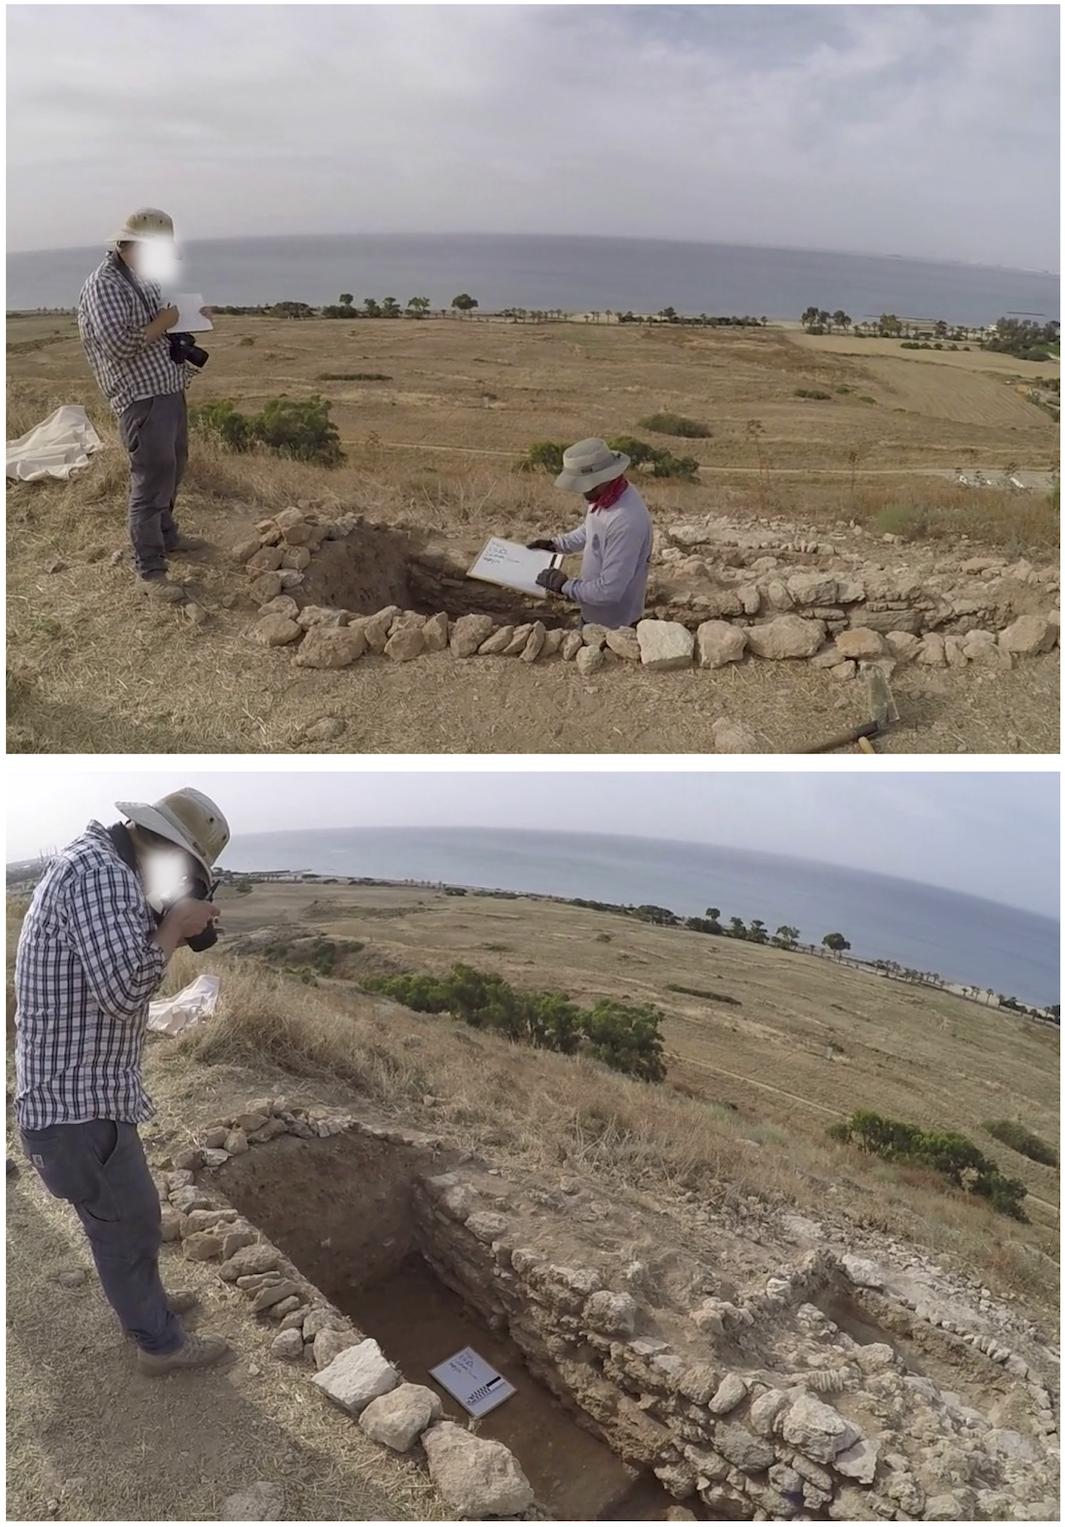
\includegraphics[keepaspectratio]{figures/photography.png}}

}

\caption{\label{fig-photography}Archaeological photography in the field
involves relating the photograph to other records about the object being
photographed.}

\end{figure}%

Moreover,\paragraphnumber{[57]} photographers were required to capture
``complete sets'' of photos, i.e.~photos of a trench opening and
closing, with and without a photo board for each instance. In this
sense, archaeological photography became just one aspect of formulaic
data-collection procedures, and was regarded with a checklist mentality.
It was common for trench supervisors to become impatient and eager to
move on to other work, while neglecting to set up their frame in a
manner that would have ensured higher visual quality. They also often
took more photos than were necessary and opted to sort through them
later to find the best ones, but this did not ensure that any of the
photos were of good quality; the photographer instead had to choose the
best of a set of poor options, which is hardly optimal (similar
observations were also made by Knoll and Carver-Kubik 2019).

Despite\paragraphnumber{[58]} difficulties working in such relatively
inconsistent and uncontrollable environments, the strong association
between photos and \emph{records of} photos contributed to a treatment
of archaeological photography as a form of data collection. This was
apparent in my observations that data management specialists, frustrated
with inconsistent or missing data in the sets of photos that they were
responsible with curating and the logs that they were responsible for
normalizing, directed fieldworkers to do photography in ways that
conformed with data management protocols.

This\paragraphnumber{[59]} was especially evident when photography was
performed by trench supervisors instead of a dedicated field
photographer, as was the case in Case A. Trench supervisors were
instructed to capture a specific set of images when triggered by certain
events, e.g., when opening and closing a trench or after identifying a
significant archaeological feature, and these instructions also told
them how to optimize the outputs of their efforts, e.g.~managing
lighting and eliminating problematic shadows. However, the significance
and value of this work was rarely communicated to the fieldworkers who
actually took the photographs. Instead, the creative acts of designing a
photography protocol, selecting and configuring equipment, and
establishing how to process relevant information about a photograph were
delegated to those who served a managerial role. Archaeological
photography was thereby directed by workflows, which are disciplined
ways of working and that involve a shift in the relative power held by
human and non-human agents involved in an activity.

More\paragraphnumber{[60]} generally, the adoption of workflows in
archaeological photography may be partially attributable to
technological change. When photography relied on film as a medium for
capturing images of archaeological entities, which was relatively scarce
and took lots of time to develop into finished photographs, photography
was a specialist activity. A sole photographer who carried specialized
instruments (digital single-lens reflex {[}DSLR{]} camera, scales, and
light meter) would be called upon to take all official photos of
noteworthy finds and features (cf. Dorrell 1994; Shanks and Svabo 2013).
But technological advances in digital photography that have become
widely available over the past two to three decades, including instant
image rendering, cheap and plentiful digital storage, fast electronic
file transfer, and reduced or eliminated cost of equipment (e.g., dark
rooms, developing fluid, flash bulbs), made it possible to reduce, and
even eliminate, the need for a specialist photographer in most
archaeological projects. Now fieldworkers may be quickly trained on the
job or be made to follow standard photography protocols using widely
available and relatively high-quality cameras, or even using cameras
integrated into their own smartphones.

Archaeological\paragraphnumber{[61]} fieldworkers can thus be made to
capture objects visually according to predefined protocols, stimulated
by certain triggering conditions, and using the cheapest approach
available. It is not necessary to waste time training photographers to
understand how a camera works and how to set up their equipment in a
manner that yields good results, when it is more efficient to delegate
these creative acts to experts who design systems and document the
operational specifications in excavation manuals that fieldworkers are
expected to follow blindly. Fieldworkers are rarely taught how a piece
of equipment works; instead, they are taught how to operate it. In other
words, embedding fieldworkers as components of the technical apparatus,
whose actions are dictated by workflows, reduces their creative agency.

That\paragraphnumber{[62]} being said, Morgan and Wright (2018) also
drew attention to the ways in which archaeological photography,
including acts of image manipulation, can enhance archaeological
understanding if performed in ways that are reminiscent of the intimate
engagements necessary to generate informative illustrations of entities
encountered during fieldwork, such as archaeological illustration, which
remains a relatively specialized activity. As a document about the
archaeological encounter, a photo must be created by someone who knows
what they have recovered and why it is significant. For this reason,
archaeological illustration also remains a constituent of archaeological
fieldwork, and has not become simply an extension of the data-management
domain. However, there have been attempts to do precisely this,
particularly through digital annotation of archaeological photographs
and certain applications of photogrammetry (Morgan and Wright 2018). But
these attempts have met resistance through the same mechanism that makes
archaeological illustration unique, namely an effort to situate these
practices as activities that primarily deal with archaeological
encounters rather than as creating simulacra of archaeological objects.

The\paragraphnumber{[63]} case of photogrammetry, also known as
structure-from-motion imaging, warrants further consideration.
Photogrammetry operates by inferring three-dimensional geometry from a
series of two-dimensional images of an object taken from multiple
overlapping perspectives. The points of overlap serve as common
reference points for construction of a unified three-dimensional model.
I observed this process at Case B, as performed by Rufus, who, aside
from being one of the project's co-directors, is a pioneering figure in
the use of photogrammetry in archaeological fieldwork settings.

Before\paragraphnumber{[64]} photogrammetric imaging could begin, it was
necessary to identify an object of interest, and for fieldworkers to
expend a great deal of effort to clear light debris and particulate
matter from all around the target object. The area was then cleared of
all equipment and personnel, save for spatial targets placed around the
object whose precise locations were later recorded with the differential
GPS (DGPS). Wielding a high-resolution digital camera, Rufus framed in
his mind the area around the object as if it were at the centre of a
conical grid. Starting in one position, he proceeded to take a series of
photos of the object, shifting his position by moving one step laterally
around the object before each shot. Once he completed the circuit around
the object, he took a step back and repeated the process, effectively
walking a series of concentric circles around the object. Afterward, he
went right up to the object and took a few more detailed photos up close
and from perspectives whose angles intersect at more acute angles. As he
moved, Rufus was wary to not cast shadows on the object of interest.
Once he captures all the photos, Chris came in with the DGPS rover and
recorded the locations of the spatial targets. These were subsequently
used to calibrate the spatial measurements and rectify the model against
local and global geographic coordinate
systems.\textsuperscript{\hyperref[sec-B4]{B4}}

After\paragraphnumber{[65]} returning to the dig house, Rufus
transferred the photos to his computer and sorted through them. He
imported them into Agisoft PhotoScan, a software suite that facilitates
``stitching together'' a 3D model from multiple constituent photographs.
He visually examined each image and discarded those that he believed
would disrupt the model based on his prior experience, which enabled him
to anticipate which input images would produce poor-quality 3D renders.
The software then identified points that various photos have in common
and inferred three-dimensional geometry based on the shifting
perspectives among them. Rufus then inspected the 3D model to determine
whether there were any smudged or imprecise areas and re-calibrated the
software parameters to account for any imperfections. He drew from his
years of practical experience, as well as deliberate and controlled
tests that applied different parameters on relatively simple toy
datasets, to guide his decisions in calibrating the
software.\textsuperscript{\hyperref[sec-B4]{B4}}

In\paragraphnumber{[66]} other words, photogrammetry involved a very
precise and intentional set of actions that Rufus coordinated in a
manner which foresaw potential issues in subsequent stages of work. He
performed his work with particular outcomes in mind, specifically the
ability to obtain a precise and georeferenced model against which object
distributions can be mapped. For Rufus, his knowledge of how the
mechanism works and his ability to assemble his own creation from basic
components and principles are what sets his work apart as a specialist
in this matter.\textsuperscript{\hyperref[sec-B5]{B5}} There exist more
general-purpose tools (i.e.~smartphone apps like 123D Catch) that enable
creation of similar-looking outputs by following a simplified set of
instructions in the app (presumably written by the app's developers),
but Rufus did not consider the people who use those tools to be
photogrammetry experts due to their lack of creative agency in the
overall process.

Interestingly,\paragraphnumber{[67]} in an unrecorded conversation Rufus
expressed his belief that photogrammetry is a fieldwork practice, rather
than something that ``digital archaeologists'' with little fieldwork
experience should perform. It is a drawn-out activity that necessitates
direct engagement and familiarity with the object of interest. In
thinking about how each stage of the photogrammetry workflow will affect
the next and eventually culminate in a compiled image, Rufus and Liz (a
very experienced trench supervisor at Case B) recognized the impacts
that their decisions made at various stages in the process had on the
final product, for example, when clearing debris or when discarding
blurry
photographs.\textsuperscript{\hyperref[sec-B6]{B6},\hyperref[sec-B7]{B7}}
Rufus values awareness of the context of creation and holding an
involved connection with the process through which the dataset is
developed.

In\paragraphnumber{[68]} all of this, a clear tension is evident with
regards to the treatment of visual media either as products that stand
in as relatively stable representations of objects of interest, or as
manifestations of cumulative archaeological engagements. Attempts to
systematize creation of visual media largely focused on the outcomes of
work, and seek ways to de-emphasize the subjective nature of
archaeological documentation so as to instill confidence in the
outcomes' immutability. This is accomplished by elevating tools as
actors that dominate human action, or by reducing people's actions as
being akin to the use of tools.

\subsection{Locating Agency in the Collection and Management of Spatial
Data}\label{locating-agency-in-the-collection-and-management-of-spatial-data}

Archaeologists\paragraphnumber{[69]} are very concerned with accounting
for spatial distributions of the objects they recover. Every artefact,
feature or interface an archaeologist encounters can be characterized in
spatial terms. Here I will describe various techniques that
archaeologists have developed to help systematize the collection and
integration of spatial information, and relate these practices to
emerging tensions pertaining to the coordination of labour and data.

A\paragraphnumber{[70]} common fieldwork practice in archaeology is the
use of site grids (Roskams 2001: 95-101), which were also employed in
the cases I observed. The purpose of site grids is to place highly
localized observations within broader integrated systems, namely the
project's geographical information system (GIS). Site grids are created
by marking a series of points in the physical landscape with
project-specific geospatial coordinates. These points may also
correspond with internationally-recognized global coordinate systems,
but projects tend to conduct day-to-day operations based on their own
grid systems. Each trench is therefore located near a point with fixed
spatial coordinates, and the trench's spatial dimensions can be inferred
by measuring distances from that fixed point. These derived locations,
whose positions are now known, can then be used to infer an extended
network of known points by measuring and calculating the differences
between the distances from target points to known points. In other
words, fieldworkers leverage the web of inferred points to determine and
record the positions of their interventions and of the things that they
recover.

In\paragraphnumber{[71]} the cases I observed, fieldworkers initially
recorded the positions of their finds in relational terms, i.e.~as
distances in relation to the fixed points from which they measure (see
Figure~\ref{fig-spatial-relational} and
Figure~\ref{fig-spatial-recording}).\textsuperscript{\hyperref[sec-A12]{A12},\hyperref[sec-B8]{B8}}
When finalizing their paperwork, they sometimes took on the task of
calculating fixed positions from the relational distances they initially
measured and recorded, but this was not really deemed as an essential
task within their purview.\textsuperscript{\hyperref[sec-A15]{A15}}
Instead, this work of converting measured distances into coordinates on
the site grid themselves was often delegated to specialists who work
with geospatial data.\textsuperscript{\hyperref[sec-B8]{B8}} This
contributed to a general distinction between the domain of fieldwork,
which was responsible for initial data-recording procedures, and the
domain of data management, which was responsible for conversioning,
formatting and cleaning data for analytical and interpretive purposes.

\begin{figure}

\centering{

\pandocbounded{\includegraphics[keepaspectratio]{figures/spatial-relational.png}}

}

\caption{\label{fig-spatial-relational}Recording spatial information in
relational terms.}

\end{figure}%

\begin{figure}

\centering{

\pandocbounded{\includegraphics[keepaspectratio]{figures/spatial-recording.png}}

}

\caption{\label{fig-spatial-recording}Recording spatial information in
the field. \textbf{A} depicts a system that measures distance in
relation to trench entities. \textbf{B} depicts a geospatial specialist
and a fieldworker determining an object's position using a digital
theodolite.}

\end{figure}%

However\paragraphnumber{[72]} this enactment of institutional boundaries
did not necessarily reflect fieldworkers' lack of interest in relating
their efforts as part of broader geospatial
networks.\textsuperscript{\hyperref[sec-A17]{A17},\hyperref[sec-A18]{A18}}
Rather, it conveyed fieldworkers' extreme sense of focus on the trenches
or grids under their direct purview. The grids established by geospatial
specialists effectively enabled field supervisors to relate their own
engagements within their respective trenches and transects to the
broader grid, in a way that required less mental overhead on their part.

Moreover,\paragraphnumber{[73]} the indirect relationships that
fieldworkers had with the formal site grid served as a way of
maintaining fieldworkers' unique perspectives on the things they
encountered. A trench was somewhat detached from the rest of the world
in the sense that a supervisor and her assistants developed their own
understanding of it and its features. They referred to specific boulders
by given names, attributed personalities to certain corners, and were
able to communicate about specific entities even while using the vaguest
of terms (i.e., ``that rock,'' ``over there,'' ``behind
you'').\textsuperscript{\hyperref[sec-A14]{A14},\hyperref[sec-A16]{A16},\hyperref[sec-A19]{A19}}
Fieldworkers felt \emph{obliged} to record formal distances between
entities and were bemused by the stock that data managers and analysts
put into these formal values.\textsuperscript{\hyperref[sec-A20]{A20}}
They dealt with the fuzzy boundaries between strata and the loose
distinctions between natural and cultural material on a day-to-day
basis, and recognized that relational associations, rather than formal
recording techniques, were better suited for capturing these aspects of
the archaeological record.

Working\paragraphnumber{[74]} with string, measuring tapes and plumbobs
allowed fieldworkers to operate in this relational manner and
communicate using the local lexicon of their trench. At the same time,
this also provided outputs that were deemed necessary to conduct a
thorough integrated analysis and to relate the self-contained sub-system
of the trench to a global spatial infrastructure.

However,\paragraphnumber{[75]} the gradual uptick in the use of precise
DGPS systems may be altering this balance. DGPS systems, such as the one
used in Case B, enable fieldworkers to determine an object's fixed
position without having to convert between as many relational
measurements. While it is true that DGPS positions are inferred, using a
rover in relation to a more sensitive GPS unit situated in a fixed
location, the people who use this system need only to measure a single
point to determine the object's position. Software handles the
conversions for them. Moreover, these off-the-shelf tools express each
position according to global coordinate systems, rather than the
project-specific grid system. Chris, who operated the DGPS for Case B,
really valued this, since it enabled him to instantly visualize the
points on maps downloaded from the web, which feature additional data
and aspects of the surrounded built landscape that he did not have to
add in himself.\textsuperscript{\hyperref[sec-B9]{B9}} The reduced
mental overhead and the enhanced ease of use encouraged the team to
record immense amounts of spatial data, and essentially all their
photographs and photogrammetric models are georeferenced as a result.

Fieldworkers\paragraphnumber{[76]} were therefore made to think of the
data they collect strictly in terms of contributing to a dataset and as
feeding into a subsequent stage of
work.\textsuperscript{\hyperref[sec-B8]{B8},\hyperref[sec-B9]{B9},\hyperref[sec-B10]{B10}}
As such, fieldworkers' labour was framed as part of a larger workflow,
which prioritizes an output in which they have no direct stake.
Fieldworkers were brought into, and fieldwork was performed in service
of, the domain of data management, rather than performing work that
granted them more creative agency.

\section{Discussion and Conclusion}\label{discussion-and-conclusion}

This\paragraphnumber{[77]} paper articulates the sociotechnical systems
that archaeologists develop and rely on to organize themselves and the
information they produce. My aim has been to demonstrate the situated
aspects of archaeological data management, and, in particular, to
highlight the distribution of creative agency across the continuum of
archaeological practice. I advance a pragmatic vision of archaeology,
which emphasizes local circumstances, experiences, and motivations as
key factors that drive scholarly communication and participation within
information commons.

Overall,\paragraphnumber{[78]} I found that the management of
archaeological data and of archaeological labour are deeply intertwined;
the systems that archaeologists have set up to help collect, organize,
combine, store, share, and reuse data all operate by controlling how
people work. Moreover, I found that the technical infrastructures that
archaeologists rely on are far from being asocial entities, and in fact
mask collaborative commitments, or norms and expectations that govern
professional relations among participating agents. Additionally, the
organizational structures that delineate roles and their corresponding
rights and responsibilities significantly influence how data are
structured and made valuable. By rendering labour as a series of
programmatic operations conducted by interchangeable components,
database managers and project managers work together to impose control
over relatively wild archaeological experiences, making their outcomes
conform to standard models.

More\paragraphnumber{[79]} specifically, in the workflows I observed,
managers operating from a centralized position of authority decided what
data to collect, how they should be collected, and how they should be
processed, integrated and stored --- all in advance of and separated
from the work itself. For instance, I observed that in archaeological
photography, fieldwork was brought under the domain of the database
apparatus, which curtailed fieldworkers' abilities to make independent
creative decisions. Data management systems and the formal data
structures that they enforce therefore served as vehicles through which
project directors centralized their control over work being done
throughout the project, and allowed them to take ownership over,
exploit, and redistribute the products of collective effort.
Archaeological data management should therefore be understood as
management in a more general sense due to its reliance on managerial
principles that enable strategic re-arrangement of agency from a
distance. These observations corroborate reflections by other
researchers, including Caraher (2019) and Thorpe (2012), who argued that
workflows transfer interpretive agency away from fieldworkers --- who
must decide what to record and how to record it --- to the system's
designers --- who implement the rulesets in consultation with project
management. The findings also correspond with similar observations in
commercial (Zorzin 2015) and community-led (Perry 2018; Mickel 2021)
archaeology, which advocate for more substantial redistribution of
creative agency throughout the archaeological process. They also support
observations by Hacıgüzeller, Taylor, and Perry (2021), who noted that
structured data such as those that emerge from workflows constitute
non-neutral and power-laden representations --- and as such, are the
outcomes of decisions to satisfy particular sets of warrants, needs and
desires.

It\paragraphnumber{[80]} must also be noted that the imbalanced
distribution of agency is a systemic phenomenon, and does not
necessarily connote a dichotomous and oppressive relationships between
managers and fieldworkers. For instance, in order to obtain consistent
data that generate outcomes which are valued by scientific enterprise,
managers must devise systems that control how fieldwork is
operationalized. As such, all decisions and actions are borne from
common systemic concerns.

Moreover,\paragraphnumber{[81]} the roles of ``manager'' and
``fieldworker'' are not fixed identities. Rather, they refer to the
actors whose work is directed and bounded by specific kinds of
objectives and by collaborative commitments that dictate their normative
relationships within the project collective. Their commonalities and
shared interests are reflected in mutually-held beliefs and value
regimes deriving from common formative experiences; specifically, their
work in roughly textured fieldwork environments, which are where most
archaeological data first emerge, are where virtually all archaeologists
learn about the norms and expectations that govern how to work and how
to capture data. Experiencing fieldwork imbues a prevalent understanding
that the information that archaeologists work with is generally rough,
tentative, fluid, and flexible.

The\paragraphnumber{[82]} systemic drive to produce concrete and
decisive data clashes with this intuitive understanding of data as
improvised outcome of messy experiences, and gives rise to an epistemic
anxiety concerning the nature of data (Huggett 2022). Archaeologists
respond to this anxiety by developing coping mechanisms, which range
from efforts to tighten control over data production, performing all
data analysis ``in house'' by those who already understand the nuances
of the data's creation, and parsing subtext of data documentation in
contexts of reuse beyond the scope of the project from which the data
derived (Batist 2024a, 2024b).

In\paragraphnumber{[83]} other words, the common cause and culture that
archaeology has maintained encourages a well-rounded and critical
assessment of how individual tasks fit within broader systems of
knowledge creation and drives resistance against attempts to atomize and
workflow the archaeological process. As such, while it may seem, in an
abstract sense, that projects impose order on all the work that falls
under their purview, archaeologists with plenty of fieldwork experience
know intrinsically that, in practice, this should be more accurately
described as an \emph{attempt} at order which is never fully achieved.
Similar undocumented acts and attitudes of resistance are prevalent
throughout the discipline, and are more acutely visible once the myth of
a frictionless and technologically-mediated archaeology is understood to
be a \emph{proposition} for one possible future, rather than an
inevitable next stage in the evolution of our discipline (cf. Huggett,
Reilly, and Lock 2018; Batist et al. 2021; Opitz et al. 2021; Caraher
2022; Huggett 2023).

So,\paragraphnumber{[84]} despite attempts to bring extreme order to
archaeological projects as concrete systems, the actual fuzzy nature of
archaeological projects shines through, and often in ways that
completely disrupt the carefully orchestrated workflows. This represents
an extension to Bowker's (1994) notion of ``infrastructural breakdown''
--- the phenomenon whereby infrastructure becomes acutely visible during
moments of disruption --- wherein I posit that when infrastructure
breaks down, the social structures and cultural experiences that hold
the technical apparatus together shine especially brightly. In my case
studies, the failures to control archaeological knowledge production
through the imposition of concrete structures reveal the discipline's
fundamental epistemic values, and demonstrate that the more things
change, the more they stay the same.

\section{Supplement A}\label{supplement-a}

\subsection{Description of Cases}\label{description-of-cases}

Case\paragraphnumber{[85]} A, which largely comprises the excavation of
a prehistoric site in Southern Europe, followed archaeologists' evolving
engagement with the information system over the course of several years.
Like many other archaeological projects, Case A's research team
composition and governance structure follows a common model, with a
director who coordinates the project, various specialists whom the
director recruited for their expertise in the interpretation of finds, a
number of trench supervisors who lead excavation and coordinate data
collection, and excavators who are usually less experienced students who
operate under the guidance of their assigned trench supervisors. It also
relies extensively on archaeological surface surveys and assessments of
the landscape to inform excavation strategies and guide interpretations
of finds. Case A addresses common underlying research questions, and its
participants compare its findings with similar work in the vicinity.
Moreover, it relies on and engages with local communities who support
the research by agreeing to excavation on their lands, while also
providing housing, food and other support to the mostly foreign research
team.

This\paragraphnumber{[86]} project serves as a useful case study that
illustrates of the pragmatic and multifaceted ways in which participants
reason and work their way through the rather mundane activities that
archaeologists commonly undertake in similar research contexts. I have
actively contributed to Case A for several years, largely performing
data management and maintenance work. This has provided me with a
privileged outlook on how team members structure information, how they
typically use data, and what circumstantial events or motivating factors
frame such concerns. I have documented how participants engage with this
project's information system over the course of three years, from 2017
to 2019. This involved visiting the project during its summer field
seasons to observe archaeological practices and to interview selected
participants. I also held interviews throughout the ``off season,'' both
remotely and in person. The project's director has also made all of the
project's documentation and records available to me for the purpose of
this research. The data I collected largely pertains to fieldwork
recording practices, processing and analysis of finds, records
management, interdisciplinary collaboration, decisions regarding writing
and publication of findings, and discussions of how data and findings
are presented, evaluated and revised among broader research communities.

My\paragraphnumber{[87]} work at Case A constituted a longer-term and
in-depth investigation of archaeological practice. My continual
participation at this project allowed me to develop an understanding of
the intricate social relations as they developed over time, and enabled
me to examine certain methods that are drawn out over the course of
several field seasons. This helped me account for how knowledge emerged
from activities distributed across time, place and circumstance.

Case\paragraphnumber{[88]} B centres on fieldwork conducted at at
excavation in the eastern Mediterranean region. This project is
generally regarded as being technologically innovative for the ways that
it has integrated novel digital tools and technologies into daily
fieldwork routines. More specifically, Case B makes use of
photogrammetry and advanced spatial recording systems in ways that
provide practical value, rather than as superfluous or experimental use
cases, which is how most other implementations of these tools and
technologies have been commonly characterized. Case B is also firmly
committed to publishing its data openly, having done so for several
years. It is sometimes showcased as an example of how to implement
`open' principles in archaeology more generally. While Case B has an
organizational structure similar to that of Case A, it is worth noting
that it is the second iteration of a project that began during the
mid-1990s. One of the two current co-directors is a former mentee of the
former co-directors. I visited this project for ten days during its 2019
summer fieldwork season. My visit largely focused on how participants
interact with information systems, how the tools that they use pose
challenges, and how participants find solutions to those problems.

My\paragraphnumber{[89]} work at Case B was more intensive, comprising a
week of interviewing and observation while archaeologists were engaging
in fieldwork. The project on which the case is based has a reputation as
an early adopter of digital technologies in fieldwork settings. This
presented me with a fresh alternative to what I observed in Case A,
which follows more traditional data management procedures. This case
therefore prompted me to focus on information management practices.

In\paragraphnumber{[90]} each case, I documented how archaeologists
perform various activities, specifically accounting for how these
actions fit into broader systems of knowledge production. Throughout all
cases I was able to capture a variety of embodied experiences and
outlooks corresponding with many roles and positions. This provides me
with insight regarding how data management infrastructures are valued
and used in a variety of contexts and by people working throughout the
continuum of archaeological practice. My conclusions are informed by the
community whose views I sought to articulate, and by my own standpoint
as a scholar of the culture and practice of science and of the media and
infrastructures that support it.

I\paragraphnumber{[91]} obtained informed consent from all individuals
included in this study in compliance with the University of Toronto's
Social Sciences, Humanities, and Education Research Ethics Board,
Protocol 34526. In order to ensure that participants could speak freely
about their personal and professional relationships while minimizing
risk to their personal and professional reputations, I committed to
refrain from publishing any personally identifying information. I refer
to all participants, affiliated organizations, and mentioned individuals
or organizations using pseudonyms. I also edited visual media to obscure
participants' faces and other information that might reveal their
identities. I also took care to edit or avoid using direct quotations
that were cited in other published work that follows a more permissive
protocol regarding the dissemination of participants' identifying
information.

\subsection{Research Participants}\label{research-participants}

Here\paragraphnumber{[92]} is a list and brief description of
individuals mentioned throughout the paper:

\begin{longtable}[]{@{}
  >{\raggedright\arraybackslash}p{(\linewidth - 4\tabcolsep) * \real{0.0238}}
  >{\raggedright\arraybackslash}p{(\linewidth - 4\tabcolsep) * \real{0.0476}}
  >{\raggedright\arraybackslash}p{(\linewidth - 4\tabcolsep) * \real{0.9286}}@{}}
\toprule\noalign{}
\endhead
\bottomrule\noalign{}
\endlastfoot
\textbf{A} & \textbf{Theo} & Commercial archaeologist, recommended to
Basil by a mutual friend. An excavator by profession, his competence
often serves as an example for the rest of the crew. He became field
director after a few years working as a trench supervisor. He is very
laid back and has a casual attitude. \\
\textbf{A} & \textbf{Jane} & One of Basil's top students, who joined the
project for one season. As a very independent and competent worker, she
took on supervisory responsibilities and stood out as an exemplary
fieldworker. \\
\textbf{B} & \textbf{Chris} & Project co-director. He is a specialist in
the archaeology of the region and a very experienced fieldworker. He
uses the project as a base for a field school, where undergraduate
students from his university learn basic fieldwork practices. \\
\textbf{B} & \textbf{Rufus} & Project co-director. As a former student
of one of the previous co-directors and a leading participant in prior
research at the site, Rufus was well suited to take the reigns when the
former directors transitioned to other research interests. Rufus is an
expert in the archaeology of the region, and an innovator in the
application of digital recording practices in archaeological
fieldwork. \\
\textbf{B} & \textbf{Liz} & Graduate student and trench supervisor who
worked with the project the previous year. Her dissertation is in part
based on data derived from this project. \\
\end{longtable}

Here\paragraphnumber{[93]} is a list and brief description of
individuals mentioned throughout Supplement B but who do not appear in
the main section of the paper:

\begin{longtable}[]{@{}
  >{\raggedright\arraybackslash}p{(\linewidth - 4\tabcolsep) * \real{0.0233}}
  >{\raggedright\arraybackslash}p{(\linewidth - 4\tabcolsep) * \real{0.0698}}
  >{\raggedright\arraybackslash}p{(\linewidth - 4\tabcolsep) * \real{0.9070}}@{}}
\toprule\noalign{}
\endhead
\bottomrule\noalign{}
\endlastfoot
\textbf{A} & \textbf{Gabe} & Geoarchaeologist attached to the project.
He initially served as field director, but his presence on this project
became sparse after he took on additional work with other research
projects elsewhere. He remained on board as a significant collaborator,
but no longer as field director. He is known for his aptitude with
statistical analysis and for being level-headed. \\
\textbf{A} & \textbf{Alfred} & Senior graduate student working at the
project for his geoarchaeology dissertation at a North American
university. He took on the role of field director while Gabe peeled back
his commitments. He is confident, with a hands-on, get-things-done
attitude. \\
\textbf{A} & \textbf{Dorothy} & Senior graduate student who oversees
palaeobotanical analysis, including sample collection and processing
protocols. \\
\textbf{A} & \textbf{Jolene} & Senior graduate student who oversees the
analysis of chipped stone for the project. She met Basil while working
at another project. \\
\textbf{A} & \textbf{Agatha} & Graduate student who serves as Jolene's
assistant. Her specialty is ground-stone artefacts but in this project
she largely performs logistical duties. \\
\textbf{A} & \textbf{Talia} & Junior faculty member who became involved
with the project as a trench supervisor after a colleague recommended
her to Basil. \\
\textbf{A} & \textbf{Lauren} & Graduate student who became involved with
the project as a trench supervisor after a colleague recommended her to
Basil. \\
\textbf{A} & \textbf{Lester} & Commercial archaeologist who became
involved with the project as a trench supervisor after Theo recommended
him to Basil. \\
\textbf{A} & \textbf{Olivia} & Commercial archaeologist who became
involved with the project as a trench supervisor after Alfred
recommended her to Basil. \\
\textbf{A} & \textbf{Ben} & One of Basil's top students, who joined as a
trench assistant. He came back the following year as a trench
supervisor. \\
\textbf{A} & \textbf{Isabelle} & Undergraduate student who joined as a
trench assistant. She works as Basil's lab assistant during the
off-season as well. \\
\textbf{B} & \textbf{Bernard} & Former co-director who has moved on to
working at other projects elsewhere in the region. He still consults
with the team currently working at Case B. \\
\textbf{B} & \textbf{Greg} & Rufus's old friend who serves as the
project's database technician. He works as a database operator at a
large commercial firm and is offering his expertise to rebuild the
project's database to more technically and professionally sound
standards. \\
\end{longtable}

\section{Supplement B}\label{supplement-b}

This\paragraphnumber{[94]} supplement contains sections of transcribed
interviews referenced throughout the paper. References are ordered by
case and by the order in which they appear. Each reference has a prefix
corresponding with the case to which it pertains.

\subsection{Case A}\label{case-a}

\subparagraph{A1}\label{sec-A1}

\textbf{Zack:}\paragraphnumber{[95]} What do you consider the most
valuable skill, that an archaeologist can have?\\
\textbf{Theo:} I don't know, how to wield a shovel and a mattock. That's
always a valuable skill. Like be able to identify something. Figure out
what's going on, dig it, and then accurately record it.\\
\textbf{Zack:} Alright.\\
\textbf{Theo:} That's the\ldots{}\\
\textbf{Zack:} That's a series of skills.\\
\textbf{Theo:} That's the essential\ldots{} like the essence of
archaeology. It's just like, you don't just sit behind a desk and write
little reports and stuff. It's like, without, you can't, you can't do
that without actually having dug before. It's im-- It's important to
know what the process of excavation is, in order to understand how,
like, what's going on.

\subparagraph{A2}\label{sec-A2}

\textbf{Zack:}\paragraphnumber{[96]} So uhm, can you please describe
your specialization or expertise, if you consider yourself to have
any?\\
\textbf{Lester:} Uhm, well I've been working professionally in
excavation, excavations for about three years now so my expertise comes
in in actual fieldwork rather than a specific discipline

\subparagraph{A3}\label{sec-A3}

\textbf{Lester:}\paragraphnumber{[97]} Well, I think it's important that
people come away from this not having been trained in the trench, given
a pickaxe and told to dig and get on with it, you know.

\subparagraph{A4}\label{sec-A4}

Had\paragraphnumber{[98]} a brief convo with Olivia as she was cleaning
up, when the corner cam died. I really {[}\ldots{]} by the mic. It was
about focus, {[}awareness?{]} of one's surroundings, being in the moment
and focusing on the task at hand. Focusing on the little things helps
her keep her organized. It is an active strategy in use. She hates that
although excavation is manual labour, it really requires you to actively
think. You can't just phase out --- illegible sentence. I mentioned my
tendency to compare excavation with tunnel vision, and noted how I think
it is somewhat flawed. She asked me if I played a musical instrument,
and I said no, and then asked if I could relate to that. She compared
these activities in order to convey the sense of being in the moment,
facing a task at hand, dealing with what is immediately in front of you,
literally and figuratively, and the satisfaction of achieving one's
goals and ticking off all the boxes. She likes to set goals, for herself
and for others.

\subparagraph{A5}\label{sec-A5}

\textbf{Lester:}\paragraphnumber{[99]} So, our first week was tough.
Very, very tough. We had a very uhh difficult trench to excavate, very
hard layers that were very difficult to physically excavate. Uhm and I
can dig for a certain extent, for a period of time in quite hot weather,
I'm used to this, for this is not a problem. But I see people that have
never approached this, attack it physically, really really attack it
physically, and not bear in mind that this is actually really difficult.
And it's not a physicality thing, it's a, it's a thought process. So
it's uhh, yes you're physically able to excavate twenty centimeters in a
day, but how are you going to feel at the end of the day? Are you going
to be able to identify the context while you're doing it? It's better to
excavate ten thoroughly than twenty in a hurry, you know? And, but the
speed will come with time. And so I've noticed this with Morris
particularly, he was quite, he's a very able archaeologist, a very good
digger, uhm but physically he's changed the way he approaches things, so
he won't go full-on that unclear now, and then expect to be able to do
it again the following morning. And then equally, the understanding is
growing, so like contextual change, uhm, I've really struggled to try
and integrate teaching into my methodologies on site, because that's not
my skillset, and not what I'm used to. But now I think we've finally
figured it, I'm involving him in the paperwork a lot more, making that a
part of the teaching process, a bit more. I think it's beneficial.

\subparagraph{A6}\label{sec-A6}

The\paragraphnumber{[100]} other cam is on Morris' head as he clears and
gardens to set up a new 5x1 trench. Comment: ``it is a weird trench''
(Morris). Slightly rhomboid, not as square-angled as intended. Morris
``catching on'' according to Lester after he asserted / referred to the
controlled environment that we constructed. One wall is extended 10cm
out in one corner, a mistake attributed to marking the rectangle on the
steep slope, lengthwise downhill. Morris also joked that the error might
be corrected by sloping the section by 10cm. This also contributed to
Lester's comment on Morris' ``catching on''. He is confident enough to
joke, and for the joke to be a good one, no less. Also interesting how
the work space shapes the trench. Supplies used to delimit the trench
are put on / near a rock in the corner. A clear space devoid of rocks is
needed. Supplies placed in the corner, on the rock, mark a boundary.
They also necessitate some clearance, 0.5-1m between them and the
delimited trench. Spoil head location is in the bushiest part, where the
cleared grass was placed. More room on small side for sieve, but more
land can be cleared too. Lester is thinking about where to put the spoil
heap. My earlier notes were of passive and seemingly assumed locations.
It turns out I was correct in my assumptions pertaining to where the
spoil heap would be located, and the reasoning behind its situation
there.

\subparagraph{A7}\label{sec-A7}

\textbf{Zack:}\paragraphnumber{[101]} Have you questioned any of the
methods you're using? Like internally but you've been afraid to ask.\\
\textbf{Jane:} I think the biggest thing that surprised me, and like now
it kinda makes more sense, but I was like, I wasn't the first person to
start digging, obviously Basil did first and then I kinda just like
watched what he did and then I started digging, and he was so rough with
like the context, like he just went at it with a triangle and then like
with a pickaxe, and I was like, like I pictured archaeology like, so
meticulous and slow with like a little brush, like I don't know, like I
guess maybe with like bones and shit you would do that because they're
more delicate, but I was like oh my god, like he's just breaking it up,
what if there's something delicate underneath? Like, that really took me
back.\\
\textbf{Zack:} But now I see you just going through it.\\
\textbf{Jane:} Yeah, yeah, now it's like, I guess cause they are\\
\textbf{Zack:} What changed your mind?\\
\textbf{Jane:} Cause I just realized there's like tools that have
survived thousands of hundreds of years. So it's like if they can
survive that then they can survive like triangles going through it, you
know? So might as well go quickly. But I think that was the kind of
thing at first that was like, what? This is kind of weird but okay.

\subparagraph{A8}\label{sec-A8}

\textbf{Ben:}\paragraphnumber{[102]} But I don't, like the paperwork and
all that, like I'm not like, I'm not, I'm not one to like be sitting at
a desk just writing all day. Like, I like to be in the trench, I like to
be doing something physical and like engaging, right? And I don't, like
reading and like articles and like scientific research and stuff, just
like, it doesn't interest me, like that much. Even like, I have to be
engaged in the topic, you know?\\
\textbf{Zack:} Yeah, yeah. I feel like you and Theo have a lot in
common.\\
\textbf{Ben:} I think so, yeah. Like Theo describes himself as like I
dig holes, and I'm like yeah, I can relate to that, man. Like I dig
holes too.

\subparagraph{A9}\label{sec-A9}

\textbf{Zack:}\paragraphnumber{[103]} So umm, I guess I've already got
your bio and all that. But I'm wondering if you could reiterate your
overall objective of your work. I mean how your work contributes to this
project.\\
\textbf{Theo:} Umm, the objective of my work\\
\textbf{Zack:} Or of your contri-- or of what you're doing here.\\
\textbf{Theo:} It's to dig holes. Dig holes.\\
\textbf{Zack:} So maybe a way to get a better answer, can you tell me
about the current season and what your current plans are, or have
been?\\
\textbf{Theo:} For this season I've been digging a big hole. Yeah, we
aim to finish it, but I doubt we will.

\subparagraph{A10}\label{sec-A10}

Liane\paragraphnumber{[104]} got in to plan the micromorph sampling. She
and Lauren looked at the section, pointed at levels, indicating which
should pertain to each context. Repositioned myself to better observe
Liane. She is actually `carving' (my own term, not hers) a block using a
flat metal instrument, I believe the metal inside of a trench handle,
which is embedded within the head, that was broken or taken off
illegible. Liane returned back with mallet and chisel. Others had to get
out of the way so she could proceed. Liane also applied gypsum plaster
to the micromorph sample. Apparently this one took longer to define than
the others. She will return tomorrow to chisel out the sample and apply
gypsum plaster to the internal face, and label it all up for further
analysis by Alfred. It needs time to dry, for now.

\subparagraph{A11}\label{sec-A11}

Small\paragraphnumber{[105]} discussion with Lauren and Ben about the
tools that archaeologists use, after I picked up the triangle and
repeated a tidbit I heard from Basil that it is supposed to be used for
wallpaper stripping. Ben noted that they were extremely useful, and was
surprised that it was not used primarily for archaeological purposes.
Also that they are exclusively used in the region due to the rocky and
baked soil.\\
She then demonstrated how difficult it is to use a trowel in thus
environment by showing how it would be typically used on a particularly
flat surface.

\subparagraph{A12}\label{sec-A12}

Theo\paragraphnumber{[106]} changed sections, and I found the illegible
word that followed very interesting. After hammering in the rebar and
vertically aligning the string, it is only level at a point that is
higher than the rebar. He told me to go grab the other rebar in the
corner, though it is massive. Tried hammering it in, but it was clear
that it would get blown over by the wind. I offered to hold it steady
but instead he told me to rummage in his bag and find a nail and masking
tape. He attached the long nail to the rebar, adding 4-5 inches to its
length. He then proceeded, with my assistance, to tie the string around
the nail, clip it on securely, and secure the line down with a rock.
Regarding securing the line down with a rock, this was a challenge for
me yesterday, as well as when I did this for the earlier section this
morning. I needed to find the right kind of rock, which was not too big,
but still dense. It needed to be not too rough, but with sharp angular
corners. This was never made explicit; after two failed attempts, first
with a large rugged rock, and then with a smaller, less rugged rock, he
picked up one and gave it to me, saying ``something like this''. I wound
the string around it, leaving some slack, and then positioned the rock
in a way that would render the line taut, by rotating it or securing it
around others.

\subparagraph{A13}\label{sec-A13}

Came\paragraphnumber{[107]} over with Theo, Maddie and Gwen present.
Maddie set up level strings around the trench\\
Theo asks Maddie to unfold long tape measure (referred to as tape). Then
asks to get in, hops in. Unfurls rolled out tape measure, aligns it
along north edge, top. They have selected the north section to draw.\\
One square on graph paper is 10cm in real life. I offer my clipboard.\\
``How deep is your trench?'', illegible it to the string.\\
``What corner is that?'' ``Southeast corner.''\\
``So that is your eastern section?'' ``Yep.''\\
Refers to line on paper: ``So this is your stable line.''\\
``I always start from the top''\\
Every 10cm, the distance from the ground to the line level is
measured.\\
Now they alternate. He holds the tape 10cm lower than before, dictates
the distances to the line.\\
Actually, he holds it to the edge of the unit, not the next 10cm (my
mistake).\\
Then Maddie connects the dots on her page, as per Nat's instructions.
She does a repeat line, like you would in a sketch, and he says ``no,
you want a solid line''.\\
Does this again for the next unit. Gets his scale ruler out to draw the
boulder, which interrupts the section in the corner. I did not see how
he used it, exactly. It looks like an unfilled portion, no texture at
all. It has been labelled as ``boulder'', written inside.\\
Dot-dash line drawn to indicate ``extrapolated'' drawings, used to draw
parts of the section where bedrock has been hit.\\
Then they do the base.\\
``It this bedrock?'' ``Yes.''\\
``Then you can do as I did here''\\
Dot-dash line drew up to the boulder, as on the base at its edge.\\
Dot-dash line then drawn on the corner, to complete the ``frame''.\\
Asked her what she thought. To her, it is exactly what is there. She
owes this to her being a visual person, is sure she can easily repeat by
herself.\\
Theo then teaches the symbols, patterns used to represent materials,
soils, sediment types.\\
He notes his own conventions as opposed to general convention, to draw
pottery and other finds that stick out of the sides.\\
Also must draw in only the big rocks. After some discussion concerning
what counts as such, Theo demonstrates which ones fit with his
description or conventional ways to define such rocks, by pointing out
which ones fit those criteria.\\
Another layer, just then drawn. It is ``wedged'' past the dot. Dangles
under the boulder, since it is somewhat extrapolated. This is not a
complete line, only sticks out of that vertical dot-dash under the
boulder.\\
Then Theo offers the tape to Gwen, who tells the measurements at the
line. Theo places his hand at the base to support the tape, since she is
slightly unsteady, and she can not bend over to look at how the bottom
aligns with the layer's edge. Theo also uses this to control where the
edge is defined.\\
Now they're drawing the rocks. First is actually a negative impression,
where a rock presumably fell out. Theo says to typically draw three
points. However in this case he suggests four to be sure. He then says
to just `eye in' the shape of the lines that connect them.\\
She does so, then indicates that her lines are less well-defined than
before, in a hesitant tone.\\
Theo procures a pencil sharpener, and sharpens it himself. He is very
careful, after some big twists, does a few smaller twists, pulling it
out and inspecting the tip each time.\\
Jess now measuring points on rocks on her own.\\
Theo says that you can use any number of points, depends on how
comfortable you are, and depends on the rock, but he prefers to use less
points and then ``draw it all in'' by eye.\\
After he packs his bag to go back, she traces over her solid lines,
defines them more strongly using her sharpened pencil. Theo offered to
come back in an hour, but Maddie insists it will take less than that.
Theo agrees.

\subparagraph{A14}\label{sec-A14}

Typical\paragraphnumber{[108]} script:\\
``At x on the horizon, it's y down''\\
Followed by an acknowledgement.\\
Sometimes a novice asks ``from what?'', or ``from the east end?'', or
``from the line?'', but once it is clarified that the reference point
remains fixed, then they instantly understand how the whole system
works. It is all about two people, working in tandem, with a commonly
understood system of communication that goes along a shared reference
point. I noticed such an ``ah-ha!'' Moment when Theo was teaching Morris
how to do this.\\
We then went to redacted trench ID, where I went down to bring some
equipment down the hill, while Theo and Jane started in redacted trench
ID. Jane is doing measurements, while Theo plots the points.\\
Jane seems very comfortable in her trench, much more than Alice
yesterday.\\
Theo is able to communicate with her, ask her questions. She also refers
to her sediment description on her contexts sheets so that Theo can
articulate ? them more appropriately. He asked whether what they just
did was the hearth and she said ``no, it's the black-brown stuff above
the hearth''. He then wrote something like that down on his drawing. He
also showed her the connected dots and asked her ``does it look
something like that?'' And she answered that it does.\\
Some other common lines:\\
``Does it go up/down left of that rock?''\\
Basically a series of relations among entities, which are described in
terms of actions that they take.\\
They ``hit the section'', ``rise/fall'', ``plateau'', ``flatten out'',
etc. In any case, the activity of the delineations is energized. Really,
the focus is on the line, or the interface. The interface moves in
relation to the reference points, that is. Moreover, it is accepted that
such activity is unclear or blurry, and that extreme precision is
pointless.

\subparagraph{A15}\label{sec-A15}

I\paragraphnumber{[109]} asked Lauren about the placement of her line
and tape measure, and she told me that it is not due to the present
circumstances - she picked that up from her first excavation, and has
been doing drawing in such a way ever since. There are several
practicalities involved. First, she finds it beneficial to measure both
upward and downward relative to the line. This is particularly useful in
deep trenches. The line is placed in an arbitrary position, where there
are few rocks at the corner, so that nails can be hammered in easily.
After one section is drawn, she can then remove one of the nails, pivot
the string around so it is on the other face of the pivot corner, and
secure it easily there. Then she must check the level on the line,
before proceeding with her measurements. She notes that setting up the
string is definitely the most time consuming, or effortful, part of
drawing.\\
This seems to have several advantages over Theo's way of doing things,
in terms of relative ease. There was definitely a lot of effort put into
securing the line, making sure it is taught, etc, since he relies on
shaky rebars, strings tied down with rocks, and an above-surface line
that blows in the wind or is at risk of being tripped over. However, he
uses the local datum as the reference point, and does not have to
measure the depth of the line. This additional set of numbers and
calculations might be an impetus for his aversion to Lauren's method,
but I have not asked him about it yet.

\subparagraph{A16}\label{sec-A16}

I\paragraphnumber{[110]} will now observe Theo and Alice draw the
sections for trench redacted trench ID. No one else is here, and Theo
expressed some confusion regarding what is going on in this trench.
Moreover, Basil can not find the paperwork for redacted trench ID, he is
on top of the hill at either redacted trench ID or redacted trench ID,
and Jane is resting back at the dig house. So it should be interesting
to see how Theo's drawing pans out with Basil's expectations.\\
He is currently setting up the illegible word, string and line levels.
It is extremely windy, so it is a bit of a challenge. As before, the
string and tape measure are clipped to the rebar that are staked into
the ground at the corners. The line is on the south section. Because of
the slope, much of the line is higher than the ground and this causes
the wind to shake it all over the place.\\
Alice on the big boulder in the southeast corner. Theo on the north
side, with graph paper, taped down to his clipboard with bandaids. Alice
calls out numbers to him as he asks them down. They called for my help
for a moment because it was too deep for Alice. Upon hearing the
elevation of the base at 1.5m along the edge, Theo illegible word and
said it is illegible word too deep, and that he would need another sheet
of paper. This wind is going to make that horrendously difficult. So
they re-prioritized, and limited their scope to the upper part that
would fit on the page.\\
I was interrupted, since my assistance was needed. I had to hold the
tape illegible words numbers to Theo. It was also challenging since no
one who actually knows the material was actually present to interpret
the stratigraphy. Basil then came by, acknowledged that this would not
be very effective due to the wind and unfamiliarity with the trench, and
instead Theo, Alice and I spent the rest of the day lugging equipment
down the hill.

\subparagraph{A17}\label{sec-A17}

\textbf{Ben:}\paragraphnumber{[111]} Oh, okay. To Basil, and I guess as
the, to the project as a whole, we want, in my trench, to find Levallois
technology or whatever, uhh cores, with Levallois characteristics.\\
\textbf{Zack:} Is that a goal that is in your mind?\\
\textbf{Ben:} Sorry?\\
\textbf{Zack:} Is that goal in your mind often?\\
\textbf{Ben:} No, well, I don't--\\
\textbf{Zack:} Sorry, I interrupted, sorry. That's what happens when I
drink, I talk too much.\\
\textbf{Ben:} Hahaha, okay umm. I guess subconsciously it would be in my
mind. I don't think I'm actively being like, oh, that's a Levallois
core, let me pick that out. Like, regardless of if it's Levallois or
not, it's gonna be picked up and put in the bag. Umm, by extension, we
want to find Levallois stuff, or I don't even know what kind of Upper
Palaeolithic or whatever, I don't know, I'm not good with those ages.
But uhh, we want to find that without, like, ruining the dating by
finding pottery or obsidian or something else. So uhh, I guess the role
of my trench is to find this, find this stuff, without finding the other
stuff that is gonna like ruin the dates for Basil.

\subparagraph{A18}\label{sec-A18}

\textbf{Zack:}\paragraphnumber{[112]} Do you, like, so, what, is there
something specifically that really piqued your interest? Like, not
necessarily like lithics, but like, or like working in the field, but
like something really specific that really, like you want to continue?
Or no? And that's fine if you don't. But is there anything that\ldots{}
what's the most exciting thing to you, if there is anything like that?\\
\textbf{Jane:} Uhh like, I'm sorry, in {[}the project{]}, you mean?\\
\textbf{Zack:} Yeah, or like things that you want to take with you.\\
\textbf{Jane:} Umm. Well I've liked, I think one of the coolest things
about working on this project is the people that like come in and out.
Like, I didn't really know that like Alfred's kind of job is like so
close to the {[}unclear{]} of archaeology. Or like meeting umm Richard,
who has like Neanderthal seafaring. It's kind of like, almost like a
consistent conference for archaeologists. Like we don't really have like
the same business opportunities that they {[}unclear{]}, so I've like
that part. I liked, I like Neanderthals, because it's kind of like the
gateway for me to, and then I get to meet those other people, so that
was, that's been exciting for me, I like doing that.\\
\textbf{Zack:} Yeah.\\
\textbf{Jane:} And like having the association with Basil. So now I can
say like, I don't know if you remember me, but I was working with Basil
Basil, like that kind of thing is important.\\
\textbf{Zack:} Yeah, it's very important.\\
\textbf{Jane:} Yeah.\\
\textbf{Ben:} I came into this, less thinking about like my future
career in anthro, and more like developing myself, so it's\ldots{}

\subparagraph{A19}\label{sec-A19}

Sam\paragraphnumber{[113]} came in to smash the big boulder. He asked,
jokingly, if it has a name, and surely enough it is named Matilda. This
is a common practice that eases the sociality, but also serves the
practical purpose of being able to identify particular objects out of
many potential candidates, i.e.~rather than referring to ``that big rock
over there'' and receiving a reply ``which one?'' with a chuckle. Also
facilitates problem solving or strategizing back at the dig house,
discussion on how to proceed.\\
Usually relatively long-lasting objects or obstructions are named. When
they are removed they are ``dead'' or ``killed''. A mini mournful
comment is sometimes made, maybe to provide a sense of closure perhaps?

\subparagraph{A20}\label{sec-A20}

Finally\paragraphnumber{[114]} asked him about his selection of rocks to
draw first. He always draws biggest first, since the smaller ones can be
more easily drawn around them.\\
Interesting that a reference point is needed for the smaller ones, but
not the bigger ones.\\
Asked him about this after he got back from the bathroom. With smaller
ones, he's just ``guesstimating''. ``I mean, you could spend hours
measuring them in, but you know, that would take hours.''\\
Sacrifice of time and effort and comfort. He is in a position to make
such decisions and there seems to be a threshold of quality, as which
point such minutia do not matter. He recognizes this, and it has come up
in our prior discussions while doing data entry for him.\\
He is meticulous, but also gets a bit fed up in the sun sometimes.\\
Anyway, the purpose according to him is to document the distinct units,
not the rocks within them. Certain large rocks are selected because they
frame the context.\\
According to Theo, ``they're important''.

\subsection{Case B}\label{case-b}

\subparagraph{B1}\label{sec-B1}

\textbf{Zack:}\paragraphnumber{[115]} Or are there certain competencies
or skills, or like, just mindsets needed?\\
\textbf{Chris:} I think, yeah, I mean I always feel like the mindset has
to be like, I will go and try to make this, make this work as best as
possible. Like kind of come up with those convenient sort of work
around, like I found a way. Here's like, here's a unclear, like
something from the national geo like geological survey, where I can just
plug in, it will plug in some coordinates that will spit uhh spit out
the correct UTM coordinates. Had to do it one by one, I think there's a
way of doing it on a mass level but I just haven't been bothering to do
that yet because I only need to do really one at a time, that's-- and
then, you know that I can plug it all into GIS anyway and then Rufus can
just flip the switch and just turn it to UTM, so it's fine. Umm. That, I
think you're just sort of like work with what you're, or kind of work
with what you've got. I mean like sort of our sieves are sort of an
example of that. The original sieves were sort of like here's what we
got, we have no money, let's just get some like little/electrical ties
and piece of janky sieve we found and just make it work with some dowel.
Like you know, it's super cheap. It's sort of like a unclear sort of
like on the fly, and you just kind of have, gonna have to do that to be
super flexible. And it's sort of like, that's my view of technology.

\subparagraph{B2}\label{sec-B2}

\textbf{Zack:}\paragraphnumber{[116]} Can you just take a minute to
explain it to me? The document that you made there?\\
\textbf{Oliver:} So, started by drawing just the outside of the square,
these lines here. Then inside, with these walls, you know, focusing on
getting the articulation on this centre wall where the pit is. Umm, so
kind of getting the bigger stones, umm just indicating that we think
there is a wall there, and then capturing the general outline of the
pit, umm, they excavated, and getting a little bit of definition as far
as how steep it is.

\subparagraph{B3}\label{sec-B3}

\textbf{Zack:}\paragraphnumber{[117]} Can I get a brief shot of the
page, what you're writing there?\\
\textbf{Chris:} Sure.\\
\textbf{Zack:} Yeah, it's just basically a photo log.\\
\textbf{Chris:} Yeah, just a photo log, just making little notes, and
then I transfer it to a, like a spreadsheet.\\
\textbf{Zack:} You keep track of the photo number? Like the file name?\\
\textbf{Chris:} Yeah, so everything, so what I do is I copy like a
reference to the image file name in that spreadsheet, and every photo,
and each photo is labelled like redacted context ID\_P1, \_P2, like for
each, each, each umm stratigraphic unit.

\subparagraph{B4}\label{sec-B4}

\textbf{Rufus:}\paragraphnumber{[118]} Okay, so if we can have just
nobody standing on this line, just cause of the shadows kicking over So
can you come on this side?\\
\textbf{Zack:} Sure, sounds good.\\
\textbf{Zack:} So the shadow was to, the shadows--\\
\textbf{Rufus:} So the basic thing with the shadows is that, if my
shadow is right here, and I take a picture, and then I take a picture
over here and my shadow has moved, the photogrammetry can't find similar
points of interest. Because it's looking for that shadow but then
suddenly that shadow's in a different position in another picture and as
far as the alignment goes it's a big mess.\\
\textbf{Zack:} Ok.\\
\textbf{Rufus:} So I always have to keep an eye on my shadow. Obviously
grasses and things like that create a problem because they're really
long and skinny and they can move one way or the other. And again, it's
for points of emphasis, for similar features on multiple pictures.\\
\textbf{Zack:} Ok.\\
\textbf{Rufus:} So when you take your pictures you have to make sure you
uhh, have enough, you do it systematically and you do it so you have
enough overlap, so you know like like 30\% per picture. I'm just gonna
move things out of the way a bit.\\
(moves some buckets)\\
\textbf{Rufus:} So the idea is you start farther out, you take pictures
around. And then you go in, take pictures in a circle, and then you go
over the object and take pictures that way.\\
\textbf{Zack:} Alright.\\
\textbf{Rufus:} So that's the, that's the goal here.\\
\textbf{Rufus:} Then after you do the big circle, the inner circle, you
just kind of go over the top and take some like random pictures to make
sure you have some extra coverage on the unit you wanna-- to make sure
you have coverage\\
\textbf{Zack:} So, when you process these, do you systematically
organize them?\\
\textbf{Rufus:} Uhh, it brings them it and it automatically aligns
them.\\
\textbf{Zack:} Oh.\\
\textbf{Rufus:} But the thing, the time consuming part uhh they call
masking, basically you're cropping out things that you don't want in
there.\\
\textbf{Zack:} Yeah.\\
\textbf{Rufus:} That takes some time. But if you do that right and run
it it'll do a good run.

\subparagraph{B5}\label{sec-B5}

\textbf{Rufus:}\paragraphnumber{[119]} Umm, but there are online places
where you can go to upload these things, and uhh my work with Mark,
quote a bit at uhh at a co-worker's project in another site, umm looking
at his information and data, he's put a lot up on file sharing sites,
like uhh, I'm trying to think of the name of some of them, I can't, but
there are places where you can upload 3D models and type a couple of key
words into it, go to this place, google it, google Pompeii and you can
see these models unclear.\\
\textbf{Zack:} Uhh one comes to mind, it's called SketchFab.\\
\textbf{Rufus:} SketchFab, that's it.\\
\textbf{Zack:} Is that it\\
\textbf{Rufus:} Exactly.\\
\textbf{Zack:} Okay.\\
\textbf{Rufus:} Yeah, SketchFab.\\
\textbf{Zack:} Uhh and, do you find that's being used extensively by
archaeologists? Or just uhh, or is, do you get a good DOI out of it? Or
is it sort of that, would it support this, what you want out of it?\\
\textbf{Rufus:} Uhh I think it's more of a, kind of just a, I mean it's
almost like an Instagram of, of 3D models. You can, you have your
profile set up, you can type key words into it, and just throw it up
there.\\
\textbf{Zack:} Mhm.\\
\textbf{Rufus:} Umm the, uhh, the, the ability to manipulate, measure,
umm isn't as great as you would want to see unclear or whatever, but
it's there, it's useable, it's umm, it's more of a, it's more of an
aesthetic thing like hey, check this out,\\
\textbf{Zack:} Yeah.\\
\textbf{Rufus:} this is what we're doing.

\subparagraph{B6}\label{sec-B6}

\textbf{Liz:}\paragraphnumber{[120]} We took out, we uhh, moved all the
vessels off of a floor in one room. And what we saw were these clusters
of certain types of artefacts on one side of the room. And then we saw a
totally different, not totally different, but a unique set of artefacts
on the other side. So this shows us that in the southern end, my theory,
right, is that there's umm a shelf on a wall that falls, right. And so
that part of the room was used for that, for storing of those types of
vessels. The other side, totally different. So, and thinking about how
you want to assess the stratigraphic unit in of itself, as, as, sort of,
a component, or umm a sort of final component of a bunch of smaller
groups, and sort of informs that.\\
\textbf{Zack:} So how did you control for that?\\
\textbf{Liz:} So we took GPS points by cluster of artefacts, which were
defined based on their spatial relationships to features around them. So
we didn't grid it. I think gridding is sort of, creates arbitrary
boundaries. So we wanted to create boundaries that could reflect
whatever use the room had in antiquity. So we did that. And then
collected artefacts, umm, and plotted them by cluster.

\subparagraph{B7}\label{sec-B7}

\textbf{Rufus:}\paragraphnumber{[121]} Anyway, uhh you go individually
photo by photo, and then you just crop out the stuff that you don't want
to be included in the processing. If you don't do that then the model
can take eight to twelve hours and then crash and it's a, it's a big
mess, just cause it's looking for all those points across that space. So
then I had to, kind of, refining your environment will allow you to, to
process something and get pretty, pretty clear. So then what we do,
obviously this is not a uhh, so in previous seasons you uhh, eighteen
for example, taken that model, this is just a report from last year. We
take that model and then export it to geo-referenced ortho-TIFF, we then
take that and create top plans based on that.

\subparagraph{B8}\label{sec-B8}

\textbf{Liz:}\paragraphnumber{[122]} Okay. So umm, when we talk of the
form we think primarily about soil and relationships, so everything on
the top is filled out, umm dealing with what types of soil are we
dealing with, and how does it compare with what's going on around it.
And of course the Harris matrix. All of the elevations and coordinates
are locked in a computer system so umm all those go in later, with the
end of the unit, umm once we get all that data, which is all used in the
GPS.\\
\textbf{Zack:} Mhm.\\
\textbf{Liz:} Umm, uhh. I like to include as much detail as possible on
procedure, so right here and a bit on the back. Umm so describing the
type of sieve, umm we have 5mm sieves here, umm and then of course water
sieving and then finds recording as we go, so make sure that nothing--\\
\textbf{Zack:} So you have a water sieve, but not here?\\
\textbf{Liz:} Uhh we don't actually have an operational one right now
but we do umm, we collected about 10 bags of soil last year that we need
to water sieve that are just waiting\\
\textbf{Zack:} But you also redundantly do it in the database, I
presume?\\
\textbf{Liz:} Yeah.\\
\textbf{Zack:} So you have both parallel records then?\\
\textbf{Liz:} Exactly. Yeah. The goal is to have them match 100\%, so
the scans of these will be matching.\\
(flips sheet over to back side)\\
\textbf{Liz:} Umm, and then our description is for discussing in more
detail the relationship between the soil and the inclusions in the
matrix that we didn't see before, umm what's different about it, how is
it umm, what is its relationship with what came before, what's its
relationship with what we're umm finding and revealing as we go. Umm,
also sort of exploring, umm, the relationship to the different features,
so walls, things like that, umm installations.\\
\textbf{Liz:} And then procedures. So like discussing types of tools
used, umm order, or sort of method and direction of excavation, umm
those kinds of things, all go on the back.\\
(flips sheet over to front side)\\
\textbf{Liz:} Umm, where a lot of the sort of interpretive and those
kinds of things. So like for like the labelling of units, I give them
something that's very very vague, that purely describes what we're
seeing, rather than interpreting what it means, so just soft fill on
that side of the trench, for example. And then in the actual, in my
trench notebook, that's where I put all of those thoughts, umm, in more
detail.\\
\textbf{Zack:} Can you show me your trench notebook, briefly? You don't
have to go into great detail into what's in the notes, but an overview,
I guess.\\
\textbf{Liz:} Yeah, so, we're excavation unit 20.\\
\textbf{Zack:} This is the front page?\\
\textbf{Liz:} This is the front page. Umm so here are umm the
coordinates of the uhh, the northing, easting and elevation of the
corners. So those obviously aren't gonna move so those are permanent.
All recorded in UTMs in 36 south. Umm, the opening elevation at the
centre. So really umm, the foundation for how we started. And then sort
of a brief sketchy Harris matrix that keeps evolving over time.\\
(turns page)\\
\textbf{Liz:} This is just a sketch plan of features in the trench, so
that I can keep the numbers straight, and keep referring back to it. Umm
and then just day by day notes, including things such as who's actually
working in the trench today, uhh what's the weather like, those kinds of
things. If someone comes to visit, I write that down, umm it's just a
way to sprint of jog your memory to sort of remember which day you're
talking about.\\
\textbf{Zack:} Do you write in prose form?\\
\textbf{Liz:} I write it in prose form, mhm. With some bullets, there
are bullet points and things like that, especially for things like
points taken, things like that, umm sketchy little things like that
about what the trench looks like at different points throughout the day,
just to keep reminding myself about what's going on. Umm and then
interpretation, so what can it possibly be, what's its possible
relationship. Even if we don't know it yet, I'll let those come out
here.\\
\textbf{Zack:} So really, so that summary, at the top of the sheet?\\
\textbf{Liz:} Yeah, in more detail, and sort of describing-- so this for
example, umm I'm not going to call it a floor on this sheet, I'll call
it a floor here.\\
\textbf{Zack:} It's more open-ended I guess?\\
\textbf{Liz:} Because it's more, yeah, it's more sort of postulating
what could be true and what could not be true. Umm, yeah.\\
\textbf{Zack:} And do you start, let's say you're starting a new trench,
do you start a new notebook?\\
\textbf{Liz:} Yeah. So each trench gets its own.\\
\textbf{Zack:} Do you, are these integrated into the database? Are they
scanned or integrated into the database at some point? Or
cross-referenced at all?\\
\textbf{Liz:} They're scanned. Umm, as far as I know they're not
cross-referenced with any particular points in the database. Umm, our
database isn't operating yet.

\subparagraph{B9}\label{sec-B9}

\textbf{Zack:}\paragraphnumber{[123]} How, it's great umm. Have there
been any specific or significant events or, events or people or uhh uhh
significant significant events or people that serves uhh umm uhh changes
that that have guided you in this direction? Uhh towards, in towards
archaeology or that have sort of pushed you into archaeology or into the
application of digital methods in archaeology?\\
\textbf{Chris:} The application of digital methods? I mean there's no,
no one or no one thing in particular. It's sort of just my own umm
thinking about the you're kinda thinking about like what would be most
effective and most most sort of streamlined umm in in in terms of in
terms of recording, tools used, things like that. Umm and sort of like I
asked around, I talked unclear, again, it's mostly under my own sort of
initiative umm.

\subparagraph{B10}\label{sec-B10}

\textbf{Zack:}\paragraphnumber{[124]} does the, does the use of such
technologies effect the ways that archaeologists work?\\
\textbf{Liz:} I mean I think so. I think it allows you to either rely on
it, and so you say well ArcGIS will tell us so we'll just leave that,
we'll plat that in, it'll be fine. Umm but also, in a, in a good way and
in a bad way, right? In a, like, let's speed up this process. And also
in a like, so maybe I can be a little bit, you know, less meticulous in
the field or something. Umm because of, this is what ArcGIS can
register. Umm it can't register finer than that, maybe, or something
like that. Umm so I think if it's the only tool that you're using, it
certainly would change uhh, yeah it would change the sort of decisions
that you make, yeah.

\section{References}\label{references}

\phantomsection\label{refs}
\begin{CSLReferences}{1}{0}
\bibitem[\citeproctext]{ref-adkins1989}
Adkins, Lesley, and Roy Adkins. 1989. \emph{Archaeological
{Illustration}}. Cambridge, UK: Cambridge University Press.

\bibitem[\citeproctext]{ref-atici2013}
Atici, Levent, Sarah Whitcher Kansa, Justin Lev-Tov, and Eric C. Kansa.
2013. {``Other {People}'s {Data}: {A Demonstration} of the {Imperative}
of {Publishing Primary Data}.''} \emph{Journal of Archaeological Method
and Theory} 20 (4): 663.
\url{https://doi.org/10.1007/s10816-012-9132-9}.

\bibitem[\citeproctext]{ref-austin2024}
Austin, Anne, Ixchel M. Faniel, Brittany Brannon, and Sarah Whitcher
Kansa. 2024. {``Improving the {Usability} of {Archaeological Data}
Through {Written Guidelines}.''} \emph{Advances in Archaeological
Practice}, January, 1--12. \url{https://doi.org/10.1017/aap.2023.38}.

\bibitem[\citeproctext]{ref-banning2020}
Banning, Edward B. 2020. {``Compilations: {Designing} and Using
Archaeological Databases.''} In \emph{The Archaeologists Laboratory},
43--58. Springer International Publishing.
\url{https://doi.org/10.1007/978-3-030-47992-3_4}.

\bibitem[\citeproctext]{ref-batist2023a}
Batist, Zachary. 2023. {``Archaeological Data Work as Continuous and
Collaborative Practice.''} PhD thesis, Toronto: University of Toronto.
\url{https://hdl.handle.net/1807/130306}.

\bibitem[\citeproctext]{ref-batist2024b}
---------. 2024a. {``Does Not Compute! {Accounting} for Social and
Situated Experiences While Integrating and Analyzing Obsidian Sourcing
Data.''} \emph{Archeologia e Calcolatori} 35 (2): 47--54.
\url{https://doi.org/10.19282/ac.35.2.2024.06}.

\bibitem[\citeproctext]{ref-batist2024a}
---------. 2024b. {``On the {Value} of {Informal Communication} in
{Archaeological Data Work}.''} \emph{Open Archaeology} 10 (1): 20240014.
\url{https://doi.org/10.1515/opar-2024-0014}.

\bibitem[\citeproctext]{ref-batist2021}
Batist, Zachary, Val Masters, Tiffany C. Torma, Michael Carter, Neal
Ferris, Isto Huvila, Seamus Ross, and Costis Dallas. 2021.
{``Figurations of {Digital Practice}, {Craft}, and {Agency} in {Two
Mediterranean Fieldwork Projects}.''} \emph{Open Archaeology} 7 (1):
1731--55. \url{https://doi.org/10.1515/opar-2020-0217}.

\bibitem[\citeproctext]{ref-beck2000}
Beck, Anthony. 2000. {``Intellectual Excavation and Dynamic Information
Management Systems.''} In \emph{On the {Theory} and {Practice} of
{Archaeological Computing}}, edited by Gary Lock and Kayt Brown, 73--88.
Oxford: Oxbow.

\bibitem[\citeproctext]{ref-berggren2015}
Berggren, Åsa, Nicolo Dell'Unto, Maurizio Forte, Scott Haddow, Ian
Hodder, Justine Issavi, Nicola Lercari, Camilla Mazzucato, Allison
Mickel, and James S. Taylor. 2015. {``Revisiting Reflexive Archaeology
at {Çatalhöyük}: {Integrating} Digital and {3D} Technologies at the
Trowel's Edge.''} \emph{Antiquity} 89 (344): 433--48.
\url{https://doi.org/10.15184/aqy.2014.43}.

\bibitem[\citeproctext]{ref-blumer1954}
Blumer, Herbert. 1954. {``What Is Wrong with Social Theory?''}
\emph{American Sociological Review} 19 (1): 3--10.
\url{https://doi.org/10.2307/2088165}.

\bibitem[\citeproctext]{ref-bowen2006}
Bowen, Glenn A. 2006. {``Grounded {Theory} and {Sensitizing
Concepts}:''} \emph{International Journal of Qualitative Methods} 5 (3):
12--23. \url{https://doi.org/10.1177/160940690600500304}.

\bibitem[\citeproctext]{ref-bowker1994}
Bowker, Geoffrey C. 1994. \emph{Science on the {Run}: {Information
Management} and {Industrial Geophysics} at {Schlumberger}, 1920-1940}.
Cambridge, MA: MIT Press.

\bibitem[\citeproctext]{ref-buccellati2017}
Buccellati, Giorgio. 2017. \emph{A {Critique} of {Archaeological
Reason}: {Structural}, {Digital}, and {Philosophical Aspects} of the
{Excavated Record}}. Cambridge University Press.

\bibitem[\citeproctext]{ref-caraher2016}
Caraher, William. 2016. {``Slow {Archaeology}: {Technology},
{Efficiency}, and {Archaeological Work}.''} In \emph{Mobilizing the
{Past} for a {Digital Future}: {The Potential} of {Digital
Archaeology}}, edited by Erik Walcek Averett, Jody Michael Gordon, and
Derek B. Counts, 421--41. Grand Forks, North Dakota: The Digital Press
at the University of North Dakota.
\url{http://digital.library.wisc.edu/1793/89898}.

\bibitem[\citeproctext]{ref-caraher2019}
---------. 2019. {``Slow {Archaeology}, {Punk Archaeology}, and the
{`{Archaeology} of {Care}'}.''} \emph{European Journal of Archaeology}
22 (3): 372--85. \url{https://doi.org/10.1017/eaa.2019.15}.

\bibitem[\citeproctext]{ref-caraher2022}
---------. 2022. {``Collaborative {Digital Publishing} in
{Archaeology}.''} In \emph{Critical {Archaeology} in the {Digital Age}:
{Proceedings} of the 12th {IEMA Visiting Scholar}'s {Conference}},
edited by Kevin Garstki, 153--63. Los Angeles, CA: Cotsen Institute of
Archaeology Press.

\bibitem[\citeproctext]{ref-carver2010}
Carver, Martin O. H. 2010. \emph{Archaeological {Investigation}}. 1st
ed. Routledge. \url{https://doi.org/10.4324/9780203523124}.

\bibitem[\citeproctext]{ref-chadwick2003}
Chadwick, Adrian. 2003. {``Post-Processualism, Professionalization and
Archaeological Methodologies. {Towards} Reflective and Radical
Practice.''} \emph{Archaeological Dialogues} 10 (1): 97--117.
\url{https://doi.org/10.1017/S1380203803001107}.

\bibitem[\citeproctext]{ref-chapman2016}
Chapman, Robert, and Alison Wylie. 2016. \emph{Evidential {Reasoning} in
{Archaeology}}. Bloomsbury Academic.

\bibitem[\citeproctext]{ref-charmaz2003}
Charmaz, Kathy. 2003. {``Grounded {Theory}: {Objectivist} and
{Constructivist Methods}.''} In \emph{Handbook of {Qualitative
Research}}, edited by Norman K. Denzin and Yvonna S. Lincoln, 3rd ed.,
249--91. Thousand Oaks, California: SAGE.

\bibitem[\citeproctext]{ref-charmaz2014}
---------. 2014. \emph{Constructing {Grounded Theory}}. 2nd ed. SAGE.

\bibitem[\citeproctext]{ref-chippindale2000}
Chippindale, Christopher. 2000. {``Capta and {Data}: {On} the {True
Nature} of {Archaeological Information}.''} \emph{American Antiquity} 65
(4): 605--12. \url{https://doi.org/10.2307/2694418}.

\bibitem[\citeproctext]{ref-crutchley2018}
Crutchley, Simon, and Peter Crow. 2018. \emph{Using {Airborne Lidar} in
{Archaeological Survey}: {The Light Fantastic}}. Historic England.

\bibitem[\citeproctext]{ref-dallas2015}
Dallas, Costis. 2015. {``Curating {Archaeological Knowledge} in the
{Digital Continuum}: {From Practice} to {Infrastructure}.''} \emph{Open
Archaeology} 1 (1): 176--207.
\url{https://doi.org/10.1515/opar-2015-0011}.

\bibitem[\citeproctext]{ref-dallas2016a}
---------. 2016. {``Digital Curation Beyond the {`{Wild} Frontier'}: {A}
Pragmatic Approach.''} \emph{Archival Science} 16 (4): 421--57.
\url{https://doi.org/10.1007/s10502-015-9252-6}.

\bibitem[\citeproctext]{ref-dorrell1994}
Dorrell, Peter G. 1994. \emph{Photography in Archaeology and
Conservation}. 2nd ed. Cambridge Manuals in Archaeology. Cambridge, U.K.
; New York: Cambridge University Press.

\bibitem[\citeproctext]{ref-drucker2011}
Drucker, Johanna. 2011. {``Humanities {Approaches} to {Graphical
Display}.''} \emph{Digital Humanities Quarterly} 5 (1).

\bibitem[\citeproctext]{ref-edgeworth1991}
Edgeworth, Matt. 1991. {``The Act of Discovery: {An} Ethnography of the
Subject-Object Relation in Archaeological Practice.''} PhD thesis,
Durham University. \url{http://etheses.dur.ac.uk/1481/}.

\bibitem[\citeproctext]{ref-edgeworth2003}
---------. 2003. \emph{Acts of Discovery: {An} Ethnography of
Archaeological Practice}. Vol. 1131. British Archaeological Reports.

\bibitem[\citeproctext]{ref-engestrom2000}
Engeström, Y. 2000. {``Activity Theory as a Framework for Analyzing and
Redesigning Work.''} \emph{Ergonomics} 43 (7): 960--74.
\url{https://doi.org/10.1080/001401300409143}.

\bibitem[\citeproctext]{ref-faniel2013}
Faniel, Ixchel, Eric C. Kansa, Sarah Whitcher Kansa, Julianna
Barrera-Gomez, and Elizabeth Yakel. 2013. {``The {Challenges} of
{Digging Data}: {A Study} of {Context} in {Archaeological Data
Reuse}.''} In \emph{Proceedings of the 13th {ACM}/{IEEE-CS Joint
Conference} on {Digital Libraries}}, 295--304. New York: ACM.
\url{https://doi.org/10.1145/2467696.2467712}.

\bibitem[\citeproctext]{ref-flick1997}
Flick, Uwe. 1997. {``The Episodic Interview. {Small} Scale Narratives as
Approach to Relevant Experiences.''} \emph{London School of Economics
Methodology Institute: Discussion Papers-Qualitative Series}.

\bibitem[\citeproctext]{ref-flick2000}
---------. 2000. {``Episodic {Interviewing}.''} In \emph{Qualitative
{Researching} with {Text}, {Image} and {Sound}}, by Martin Bauer and
George Gaskell, 76--92. London: SAGE Publications Ltd.
\url{https://doi.org/10.4135/9781849209731.n5}.

\bibitem[\citeproctext]{ref-gero1985}
Gero, Joan M. 1985. {``Socio-{Politics} and the {Woman-at-Home
Ideology}.''} \emph{American Antiquity} 50 (2): 342--50.
\url{https://doi.org/10.2307/280492}.

\bibitem[\citeproctext]{ref-gero1994}
---------. 1994. {``Excavation {Bias} and the {Woman} at {Home
Ideology}.''} \emph{Archeological Papers of the American Anthropological
Association} 5 (1): 37--42.
\url{https://doi.org/10.1525/ap3a.1994.5.1.37}.

\bibitem[\citeproctext]{ref-gero1996}
---------. 1996. {``Archaeological Practice and Gendered Encounters with
Field Data.''} \emph{Gender and Archaeology}, 251--80.

\bibitem[\citeproctext]{ref-goodwin1994}
Goodwin, Charles. 1994. {``Professional {Vision}.''} \emph{American
Anthropologist} 96 (3): 606--33.
\url{https://doi.org/10.1525/aa.1994.96.3.02a00100}.

\bibitem[\citeproctext]{ref-goodwin2010}
---------. 2010. {``Things and Their Embodied Environments.''} In
\emph{The Cognitive Life of Things: {Recasting} the Boundaries of the
Mind}, edited by Lambros Malafouris and Colin Renfrew, 103--20.
Cambridge: McDonald Institute of Archaeological Research.

\bibitem[\citeproctext]{ref-griffiths2007}
Griffiths, Nick, Anne Jenner, and Christine Wilson. 2007. \emph{Drawing
Archaeological Finds: A Handbook}. Revised. London: Archetype
Publications.

\bibitem[\citeproctext]{ref-gupta2023}
Gupta, Neha, Andrew Martindale, Kisha Supernant, and Michael Elvidge.
2023. {``The {CARE Principles} and the {Reuse}, {Sharing}, and
{Curation} of {Indigenous Data} in {Canadian Archaeology}.''}
\emph{Advances in Archaeological Practice} 11 (1): 76--89.
\url{https://doi.org/10.1017/aap.2022.33}.

\bibitem[\citeproctext]{ref-haciguzeller2021}
Hacıgüzeller, Piraye, James Stuart Taylor, and Sara Perry. 2021. {``On
the {Emerging Supremacy} of {Structured Digital Data} in {Archaeology}:
{A Preliminary Assessment} of {Information}, {Knowledge} and {Wisdom
Left Behind}.''} \emph{Open Archaeology} 7 (1): 1709--30.
\url{https://doi.org/10.1515/opar-2020-0220}.

\bibitem[\citeproctext]{ref-hamilton2000}
Hamilton, Carolyn. 2000. {``Faultlines: {The} Construction of
Archaeological Knowledge at {Catalhöyük}.''} In \emph{Towards Reflexive
Method in Archaeology : The Example at {Çatalhöyük}}, edited by Ian
Hodder, 119--27. Cambridge: McDonald Institute for Archaeological
Research.

\bibitem[\citeproctext]{ref-hodder2000}
Hodder, Ian, ed. 2000. \emph{Towards Reflexive Method in Archaeology:
{The} Example at {Çatalhöyük}}. Cambridge, UK: McDonald Institute for
Archaeological Research.

\bibitem[\citeproctext]{ref-huggett2018}
Huggett, Jeremy. 2018. {``Reuse {Remix Recycle}: {Repurposing
Archaeological Digital Data}.''} \emph{Advances in Archaeological
Practice} 6 (2): 93--104. \url{https://doi.org/10.1017/aap.2018.1}.

\bibitem[\citeproctext]{ref-huggett2022}
---------. 2022. {``Data {Legacies}, {Epistemic Anxieties}, and {Digital
Imaginaries} in {Archaeology}.''} \emph{Digital} 2 (2): 267--95.
\url{https://doi.org/10.3390/digital2020016}.

\bibitem[\citeproctext]{ref-huggett2023a}
---------. 2023. {``Deconstructing the {Digital Infrastructures
Supporting Archaeological Knowledge}.''} \emph{Current Swedish
Archaeology} 31:11--38. \url{https://doi.org/10.37718/CSA.2023.01}.

\bibitem[\citeproctext]{ref-huggett2018a}
Huggett, Jeremy, Paul Reilly, and Gary Lock. 2018. {``Whither {Digital
Archaeological Knowledge}? {The Challenge} of {Unstable Futures}.''}
\emph{Journal of Computer Applications in Archaeology} 1 (1): 42--54.
\url{https://doi.org/10.5334/jcaa.7}.

\bibitem[\citeproctext]{ref-hutchins1995}
Hutchins, Edwin. 1995. {``How a {Cockpit Remembers Its Speeds}.''}
\emph{Cognitive Science} 19 (3): 265--88.
\url{https://doi.org/10.1207/s15516709cog1903_1}.

\bibitem[\citeproctext]{ref-huvila2011}
Huvila, Isto. 2011. {``Being Formal and Flexible: Semantic Wiki as an
Archaeological e-Science Infrastructure.''} In \emph{Revive the {Past}:
{Proceeding} of the 39th {Conference} on {Computer Applications} and
{Quantitative Methods} in {Archaeology}, {Beijing}}, 186--97.

\bibitem[\citeproctext]{ref-huvila2016}
---------. 2016. {``"{If We Just Knew Who Should Do It}", or the {Social
Organization} of the {Archiving} of {Archaeology} in {Sweden}.''}
\emph{Information Research: An International Electronic Journal} 21 (2):
n2.

\bibitem[\citeproctext]{ref-huvila2022}
---------. 2022. {``Improving the Usefulness of Research Data with
Better Paradata.''} \emph{Open Information Science} 6 (1): 28--48.
\url{https://doi.org/10.1515/opis-2022-0129}.

\bibitem[\citeproctext]{ref-huvila2023a}
Huvila, Isto, Olle Sköld, and Lisa Andersson. 2023.
{``Knowing-in-{Practice}, {Its Traces} and {Ingredients}.''} In
\emph{The {Posthumanist Epistemology} of {Practice Theory}:
{Re-imagining Method} in {Organization Studies} and {Beyond}}, edited by
Michela Cozza and Silvia Gherardi, 37--69. Cham: Springer Nature
Switzerland. \url{https://doi.org/10.1007/978-3-031-42276-8_2}.

\bibitem[\citeproctext]{ref-kansa2013}
Kansa, Eric C., and Sarah Whitcher Kansa. 2013. {``We {All Know That} a
14 {Is} a {Sheep}: {Data Publication} and {Professionalism} in
{Archaeological Communication}.''} \emph{Journal of Eastern
Mediterranean Archaeology and Heritage Studies} 1 (1): 88--97.
\url{https://doi.org/10.1353/ema.2013.0007}.

\bibitem[\citeproctext]{ref-khazraee2013}
Khazraee, Emad. 2013. {``Information Recording in Archaeological
Practice: {A} Socio-Technical Perspective,''} February.
\url{https://doi.org/10.9776/13246}.

\bibitem[\citeproctext]{ref-knoll2019}
Knoll, Michelle K., and A. Carver-Kubik. 2019. {``In-{Field Digital
Photography} and the {Curation} of {Associated Records}: {Not All Prints
Are Created Equal}.''} \emph{Advances in Archaeological Practice} 7 (3):
302--10. \url{https://doi.org/10.1017/aap.2019.17}.

\bibitem[\citeproctext]{ref-knorrcetina1999}
Knorr Cetina, Karin. 1999. \emph{Epistemic {Cultures}: {How} the
{Sciences Make Knowledge}}. Harvard University Press.

\bibitem[\citeproctext]{ref-knorrcetina2001}
---------. 2001. {``Objectual Practice.''} In \emph{The {Practice Turn}
in {Contemporary Theory}}, edited by Theodore R. Schatzki, Karin Knorr
Cetina, and Eike von Savigny, 175--88. London; New York: Routledge.

\bibitem[\citeproctext]{ref-delaet2000}
Laet, Marianne de, and Annemarie Mol. 2000. {``The {Zimbabwe Bush Pump}:
{Mechanics} of a {Fluid Technology}.''} \emph{Social Studies of Science}
30 (2): 225--63. \url{https://doi.org/10.1177/030631200030002002}.

\bibitem[\citeproctext]{ref-leontev1974}
Leont'ev, A. N. 1974. {``The {Problem} of {Activity} in {Psychology}.''}
\emph{Soviet Psychology} 13 (2): 4--33.
\url{https://doi.org/10.2753/RPO1061-040513024}.

\bibitem[\citeproctext]{ref-lucas2001a}
Lucas, Gavin. 2001. {``Destruction and the {Rhetoric} of
{Excavation}.''} \emph{Norwegian Archaeological Review} 34 (1): 35--46.
\url{https://doi.org/10.1080/00293650119347}.

\bibitem[\citeproctext]{ref-lucas2012}
---------. 2012. \emph{Understanding the {Archaeological Record}}.
Cambridge University Press.

\bibitem[\citeproctext]{ref-lucas2019}
---------. 2019. \emph{Writing the Past: {Knowledge} and Literary
Production in Archaeology}. Abingdon, Oxon ; New York, NY: Routledge.

\bibitem[\citeproctext]{ref-lukas2018}
Lukas, Dominik, Claudia Engel, and Camilla Mazzucato. 2018. {``Towards a
{Living Archive}: {Making Multi Layered Research Data} and {Knowledge
Generation Transparent}.''} \emph{Journal of Field Archaeology} 43
(October):S19--30. \url{https://doi.org/10.1080/00934690.2018.1516110}.

\bibitem[\citeproctext]{ref-martinez-del-pozo2013}
Martínez-del-Pozo, José-Ángel, Victorino Mayoral-Herrera, and Pedro
Ortiz-Coder. 2013. {``Creating and {Analysing Digital Terrain Models}
for {Archaeological Research}.''} In \emph{Good {Practice} in
{Archaeological Diagnostics}: {Non-invasive Survey} of {Complex
Archaeological Sites}}, edited by Cristina Corsi, Božidar Slapšak, and
Frank Vermeulen, 227--43. Natural {Science} in {Archaeology}. Cham:
Springer International Publishing.
\url{https://doi.org/10.1007/978-3-319-01784-6_13}.

\bibitem[\citeproctext]{ref-maryl2020}
Maryl, Maciej, Costis Dallas, Jennifer Edmond, Jessie Labov, Ingrida
Kelpšienė, Michelle Doran, Marta Kołodziejska, and Klaudia Grabowska.
2020. {``A {Case Study Protocol} for {Meta-Research} into {Digital
Practices} in the {Humanities}.''} \emph{Digital Humanities Quarterly}
14 (3).
\url{https://www.digitalhumanities.org/dhq/vol/14/3/000477/000477.html}.

\bibitem[\citeproctext]{ref-mcpherron2005}
McPherron, Shannon J. P. 2005. {``Artifact Orientations and Site
Formation Processes from Total Station Proveniences.''} \emph{Journal of
Archaeological Science} 32 (7): 1003--14.
\url{https://doi.org/10.1016/j.jas.2005.01.015}.

\bibitem[\citeproctext]{ref-mickel2021}
Mickel, Allison. 2021. \emph{Why {Those Who Shovel Are Silent}: {A
History} of {Local Archaeological Knowledge} and {Labor}}. University
Press of Colorado. \url{https://doi.org/10.5876/9781646421152}.

\bibitem[\citeproctext]{ref-mickel2015b}
Mickel, Allison, and Elijah Meeks. 2015. {``Networking the Teams and
Texts of Archaeological Research at {Çatalhöyük}.''} In \emph{Assembling
{Çatalhöyük}}, edited by Ian Hodder and Arkadiusz Marciniak, 25--42.
Routledge.

\bibitem[\citeproctext]{ref-morgan2021}
Morgan, Colleen, Helen Petrie, Holly Wright, and James Stuart Taylor.
2021. {``Drawing and {Knowledge Construction} in {Archaeology}: {The
Aide Mémoire Project}.''} \emph{Journal of Field Archaeology} 46 (8):
614--28. \url{https://doi.org/10.1080/00934690.2021.1985304}.

\bibitem[\citeproctext]{ref-morgan2018}
Morgan, Colleen, and Holly Wright. 2018. {``Pencils and {Pixels}:
{Drawing} and {Digital Media} in {Archaeological Field Recording}.''}
\emph{Journal of Field Archaeology} 43 (2): 136--51.
\url{https://doi.org/10.1080/00934690.2018.1428488}.

\bibitem[\citeproctext]{ref-nicolini2009}
Nicolini, Davide. 2009. {``Zooming {In} and {Out}: {Studying Practices}
by {Switching Theoretical Lenses} and {Trailing Connections}.''}
\emph{Organization Studies} 30 (12): 1391--1418.
\url{https://doi.org/10.1177/0170840609349875}.

\bibitem[\citeproctext]{ref-olson2013}
Olson, Brandon R., William Caraher, David K. Pettegrew, and R. Scott
Moore. 2013. {``The {Pyla-Koutsopetria Archaeological Project}: {A
Preliminary Report} of {Excavations} at {Pyla-Viglia}, a {Fortified
Settlement Dating} to the {Hellensitic Era}.''} \emph{Journal of Ancient
Egyptian Interconnections} 5 (3): 74--82.
\url{https://doi.org/10.2458/azu_jaei_v05i3_olson}.

\bibitem[\citeproctext]{ref-opitz2021}
Opitz, Rachel, Colleen Strawhacker, Philip Buckland, Jackson Cothren,
Tom Dawson, Andrew Dugmore, George Hambrecht, et al. 2021. {``A
{Lockpick}'s {Guide} to {dataARC}: {Designing Infrastructures} and
{Building Communities} to {Enable Transdisciplinary Research}.''}
\emph{Internet Archaeology} 56 (October).
\url{https://doi.org/10.11141/ia.56.15}.

\bibitem[\citeproctext]{ref-perry2018}
Perry, Sara. 2018. {``Why {Are Heritage Interpreters Voiceless} at the
{Trowel}'s {Edge}? {A Plea} for {Rewriting} the {Archaeological
Workflow}.''} \emph{Advances in Archaeological Practice} 6 (3): 212--27.
\url{https://doi.org/10.1017/aap.2018.21}.

\bibitem[\citeproctext]{ref-petrosyan2021}
Petrosyan, Artur, Hayk Azizbekyan, Boris Gasparyan, Roberto Dan, Arsen
Bobokhyan, and Mariam Amiryan. 2021. {``Foregrounding {Daily Data
Collection} on {Archaeological Fieldwork}.''} \emph{Advances in
Archaeological Practice} 9 (4): 402--14.
\url{https://doi.org/10.1017/aap.2021.30}.

\bibitem[\citeproctext]{ref-politis2001}
Politis, Gustavo. 2001. {``On Archaeological Praxis, Gender Bias and
Indigenous Peoples in {South America}.''} \emph{Journal of Social
Archaeology} 1 (1): 90--107.
\url{https://doi.org/10.1177/146960530100100107}.

\bibitem[\citeproctext]{ref-ragin1992}
Ragin, Charles C. 1992. {``Casing and the Process of Social Research.''}
In \emph{What Is a {Case}? {Exploring} the {Foundations} of {Social
Inquiry}}, edited by Charles C. Ragin and Howard S. Becker, 217--26.
Cambridge University Press New York.

\bibitem[\citeproctext]{ref-richards-rissetto2019}
Richards-Rissetto, Heather, and Kristin Landau. 2019.
{``Digitally-{Mediated Practices} of {Geospatial Archaeological Data}:
{Transformation}, {Integration}, \& {Interpretation}.''} \emph{Journal
of Computer Applications in Archaeology} 2 (1): 120--35.
\url{https://doi.org/10.5334/jcaa.30}.

\bibitem[\citeproctext]{ref-roskams2001}
Roskams, Steve. 2001. \emph{Excavation}. Cambridge Manuals in
Archaeology. Cambridge, UK: Cambridge University Press.

\bibitem[\citeproctext]{ref-rousseleau2015}
Rousseleau, Raphaël. 2015. {``Lire La Terre, Truelle En Main. {Une}
Ethnographie de La Fouille Archéologique Amateure.''}
\emph{Ethnographiques. Org} 31.
\url{https://www.ethnographiques.org/2015/Rousseleau}.

\bibitem[\citeproctext]{ref-saldana2011}
Saldaña, Johnny. 2011. \emph{Fundamentals of Qualitative Research}.
Understanding Qualitative Research. New York: Oxford University Press.

\bibitem[\citeproctext]{ref-sandoval2020}
Sandoval, Gustavo. 2020. {``The {Relevance} of {Çatalhöyük Reflexive
Diaries}.''} In \emph{New {Frontiers} in {Archaeology} : {Proceedings}
of the {Cambridge Annual Student Archaeology Conference} 2019}.
Cambridge, UK: Archaeopress Publishing.

\bibitem[\citeproctext]{ref-shanks2013}
Shanks, Michael, and Connie Svabo. 2013. {``Archaeology and Photography:
{A} Pragmatology.''} In \emph{Reclaiming {Archaeology}: {Beyond} the
{Tropes} of {Modernity}}, edited by Alfredo González-Ruibal, 89--102.
London; New York: Routledge.

\bibitem[\citeproctext]{ref-star1989}
Star, Susan Leigh, and James R. Griesemer. 1989. {``Institutional
{Ecology}, '{Translations}' and {Boundary Objects}: {Amateurs} and
{Professionals} in {Berkeley}'s {Museum} of {Vertebrate Zoology},
1907-39.''} \emph{Social Studies of Science} 19 (3): 387--420.
\url{https://doi.org/10.1177/030631289019003001}.

\bibitem[\citeproctext]{ref-suchman2007}
Suchman, Lucy. 2007. \emph{Human-Machine Reconfigurations: Plans and
Situated Actions}. 2nd ed. Cambridge University Press.

\bibitem[\citeproctext]{ref-taylor2018}
Taylor, James, Justine Issavi, Åsa Berggren, Dominik Lukas, Camilla
Mazzucato, Burcu Tung, and Nicoló Dell'Unto. 2018. {``'{The Rise} of the
{Machine}': The Impact of Digital Tablet Recording in the Field at
{Çatalhöyük}.''} \emph{Internet Archaeology} 47.
\url{https://doi.org/10.11141/ia.47.1}.

\bibitem[\citeproctext]{ref-taylor2015}
Taylor, James, Dominik Lukas, and Åsa Berggren. 2015. {``Digital
Recording and Reflexive Methodology at {Çatalhöyük}.''} Edited by Scott
D. Haddow. \emph{Çatalhöyük 2015 Archive Report}, 195--96.

\bibitem[\citeproctext]{ref-thorpe2012}
Thorpe, Reuben. 2012. {``Often {Fun}, {Usually Messy}: {Fieldwork},
{Recording} and {Higher Orders} of {Things}.''} In \emph{Reconsidering
{Archaeological Fieldwork}: {Exploring On-Site Relationships Between
Theory} and {Practice}}, edited by Hannah Cobb, Harris Harris Oliver J.
T., Cara Jones, and Philip Richardson, 31--52. Springer, Boston, MA.
\url{https://doi.org/10.1007/978-1-4614-2338-6_3}.

\bibitem[\citeproctext]{ref-torterat2020}
Torterat, Gwendoline. 2020. {``Être Attentif En Archéologie: {Modalités}
de Transmission d'un « Savoir Voir » Entre Experts Et Novices Sur Un
Site Paléolithique.''} \emph{Revue d'anthropologie Des Connaissances} 14
(3). \url{https://doi.org/10.4000/rac.10867}.

\bibitem[\citeproctext]{ref-waagen2019}
Waagen, Jitte. 2019. {``New Technology and Archaeological Practice.
{Improving} the Primary Archaeological Recording Process in Excavation
by Means of {UAS} Photogrammetry.''} \emph{Journal of Archaeological
Science} 101 (January):11--20.
\url{https://doi.org/10.1016/j.jas.2018.10.011}.

\bibitem[\citeproctext]{ref-witzel2000}
Witzel, Andreas. 2000. {``The Problem-Centered Interview.''} \emph{Forum
Qualitative Sozialforschung / Forum: Qualitative Social Research} 1 (1).
\url{https://doi.org/10.17169/fqs-1.1.1132}.

\bibitem[\citeproctext]{ref-wylie1989}
Wylie, Alison. 1989. {``Archaeological {Cables} and {Tacking}: {The
Implications} of {Practice} for {Bernstein}'s {`{Options Beyond
Objectivism} and {Relativism}'}.''} \emph{Philosophy of the Social
Sciences} 19 (1): 1--18.
\url{https://doi.org/10.1177/004839318901900101}.

\bibitem[\citeproctext]{ref-wylie2003}
---------. 2003. {``Why {Standpoint Matters}.''} In \emph{Science and
{Other Cultures}: {Issues} in {Philosophies} of {Science} and
{Technology}}, edited by Robert Figueroa and Sandra G. Harding, 26--48.
Routledge.

\bibitem[\citeproctext]{ref-wylie2010}
---------. 2010. {``Archaeological {Facts} in {Transit}: {The}
{`{Eminent Mounds}'} of {Central North America}.''} In \emph{How {Well
Do Facts Travel}? {The Dissemination} of {Reliable Knowledge}}, edited
by Peter Howlett and Mary S. Morgan, 301--22. Cambridge, UK: Cambridge
University Press.

\bibitem[\citeproctext]{ref-wylie2017}
---------. 2017. {``How {Archaeological Evidence Bites Back}:
{Strategies} for {Putting Old Data} to {Work} in {New Ways}.''}
\emph{Science, Technology, \& Human Values} 42 (2): 203--25.
\url{https://doi.org/10.1177/0162243916671200}.

\bibitem[\citeproctext]{ref-yarrow2008}
Yarrow, Thomas. 2008. {``In {Context}: {Meaning}, {Materiality} and
{Agency} in the {Process} of {Archaeological Recording}.''} In
\emph{Material {Agency}: {Towards} a {Non-Anthropocentric Approach}},
edited by Carl Knappett and Lambros Malafouris, 121--37. Boston, MA:
Springer. \url{https://doi.org/10.1007/978-0-387-74711-8_7}.

\bibitem[\citeproctext]{ref-zorzin2015}
Zorzin, Nicolas. 2015. {``Dystopian {Archaeologies}: {The
Implementation} of the {Logic} of {Capital} in {Heritage Management}.''}
\emph{International Journal of Historical Archaeology} 19 (4): 791--809.
\url{https://doi.org/10.1007/s10761-015-0315-4}.

\end{CSLReferences}

\subsection{Acknowledgments}\label{acknowledgments}

I\paragraphnumber{[125]} extend warm thanks to Costis Dallas, Matt
Ratto, Ted Banning, Jeremy Huggett and Ed Swenson for supervising my
work and providing critical feedback as I conducted my doctoral
research, which this paper is based upon. I am also very grateful to the
peer-reviewers for their constructive evaluation, including the
anonymous reviewers who reviewed previous iterations of this work. Of
course, this work would not have been possible without the anonymous
research participants who allowed me to observe and interview them as
they worked, and to articulate their actions and outlooks.

\subsection{Funding}\label{funding}

This\paragraphnumber{[126]} work is derived from the author's doctoral
dissertation, \emph{Archaeological data work as continuous and
collaborative practice} (Batist 2023), which was supported by the
Canadian Social Sciences and Humanities Research Council Doctoral
Fellowship (Award ID: 752-2019-2233).

\subsection{Competing Interests}\label{competing-interests}

The\paragraphnumber{[127]} author states no conflicts of interest.

\subsection{Author Contribution}\label{author-contribution}

Zachary\paragraphnumber{[128]} Batist is the sole author of this work.
He defined the scope of the study and identified suitable cases for
inclusion, collected and processed all data, performed analysis,
interpreted the findings, created all the figures, and wrote the paper.

\subsection{Informed Consent}\label{informed-consent}

Informed\paragraphnumber{[129]} consent has been obtained from all
individuals included in this study, in compliance with the University of
Toronto's Social Sciences, Humanities, and Education Research Ethics
Board, Protocol 34526.

\subsection{Data Availability
Statement}\label{data-availability-statement}

The\paragraphnumber{[130]} data generated and analyzed during the
current study are included in this published article's supplementary
files.

\subsection{Author Bio}\label{author-bio}

Zachary\paragraphnumber{[131]} Batist obtained his PhD from the
University of Toronto's Faculty of Information. His research explores
the collaborative commitments inherent throughout archaeological
practice, especially relating to data management and the constitution of
information commons. He currently works as a Postdoctoral Researcher at
the Department of Epidemiology, Biostatistics and Occupational Health in
the School of Public and Global Health at McGill University, where he
investigates the collaborative, technical and administrative structures
that scaffold data harmonization in epidemiological research.




\end{document}
